\chapter{Evaluation and Results} \label{chap:evaluation}
%One liability of image-based rendering systems is the lack of a consistent  framework within which to judge the validity of the results. plenoptic modeling: an image-based rendering system mcmillan
Unfortunately, there are no publicly available benchmarks for 360\degree image synthesis with two degrees of freedom without 3D geometry, as not many methods exist that try to achieve this. Since the approach presented in Chapter~\ref{chap:implementation} is a first, basic attempt at solving this problem, this chapter presents a basic evaluation of the algorithm, based on mathematically calculable error metrics. These metrics measure the accuracy of a synthesized image compared to the ground truth and are used to assess the effect of a limited number of parameters.
%Furthermore, it compares the results of regular blending, flow-based blending, and a na\"ive baseline algorithm to analyze whether, and in which cases an improvement could be achieved.

First, possible parameters are discussed (Section~\ref{sec:params}), followed by the presentation of the evaluation methodology (Section~\ref{sec:eval_methodology}). Then a limit evaluation is performed on virtually generated scenes to explore the limits of the algorithm in a controlled environment (Section~\ref{sec:limit_eval}). Based on the knowledge gained in the limit evaluation, a proof-of-concept evaluation is performed on real scenes (Section~\ref{sec:pof_eval}). Finally, the aggregate evaluation findings are discussed (Section~\ref{sec:discussion}).

%First the evaluation methodology is presented, outlining how the effects of a parameter are measured and evaluated. Then, the limits of the algorithm are explored using virtual scenes. With the information gleaned from this limit evaluation, the parameters are chosen for a proof-of-concept evaluation using real scenes. The results and limitations are then discussed\ldots

%- what is a scenario what is a scene
%- not performance
%- konkreter
%- wie gut koennen szenen synthetisiert werden
%- scope: basic evaluation of mathematically measurable values (no human perception)
%- these datasets could be used in the future to compare different algorithms

\section{Parameters} \label{sec:params}
Before defining the parameters to test in the limitation and proof-of-concept evaluations, this section gives an overview of possible parameters in the context of the 2~DoF algorithm presented in Chapter~\ref{chap:implementation}.
The 2~DoF algorithm already makes a few assumptions, for example the constraint to the viewpoint plane, the fact that the scene is static, and more (stated in Section \ref{sec:approach} on page \pageref{sec:approach}). These assumptions are upheld in the evaluation, as they are prerequisite to the function of the algorithm.
\todo{define performance as accuracy of results based on error metrics}

The remaining parameters (that are not constrained by the assumptions) can be divided into two categories: 
\begin{description}
    \item [Internal parameters] i.e.\ based within the algorithm, such as the blending type and the selection of input viewpoints
    \item [External parameters] i.e.\ based on the properties of the captured scene, such as the viewpoint density, or the geometry of the scene.
\end{description}      

The internal parameters can be modified after the scene has been captured, the external ones cannot.  The most prominent internal parameters based on the implementation from Chapter~\ref{chap:implementation} are:

\begin{itemize}
  \item the location of synthesized points within the scene (near walls, objects, etc)
  \item the location of synthesized points relative to the captured points
  \item the blending type, i.e.\ flow-based blending or deviation-angle-based knn blending (``regular blending'')
%  \item the selection of input viewpoints from the available captured viewpoints
  \item the optical flow algorithm used for flow-based blending
\end{itemize}

There are more internal parameters that could theoretically be modified, such as the knn blending function (the inverse sigmoid function on page~\pageref{eq:sigmoid}), or the method of approximation for 2~DoF in flow-based blending (page~\pageref{subsec:2dof_flow-based}), but these will be assumed immutable for this evaluation, as the variation of these parameters would require developing new functions, which would be outside the scope of this thesis.

As for the possible external parameters, the number of different possible scenes is infinite, but the assumed key parameters are:
\begin{itemize}
  \item type of scene (outdoor, indoor, etc) \ar size and shape of scene
  \item objects within the scene
  \item density of captured viewpoints
  \item distribution of captured viewpoints
\end{itemize}

External parameters such as the camera settings (e.g. aperture, shutter speed, white balance) and the lighting throughout the scene are not considered; it is assumed that all the captures have the same camera settings and the white balance is comparable throughout the scene. Furthermore, the evaluation is restricted to indoor scenes of approximately $25m^2$. This reduces the parameter space significantly, since the fact that indoor scenes tend to be enclosed by walls enforces a maximal distance of objects to the camera.

The evaluation presented in this thesis aims to examine the effects of a few select internal and external parameters, instead of exhaustively examining all of them. In order to do this, a \emph{scenario} is designed for each selected parameter that attempts to demonstrate the effect of this parameter on the accuracy of the result. Limiting the evaluation to specific scenarios reduces the testing space but might also lead to missing some interactions between parameters. This is acceptable, since the evaluation does not aim to be comprehensive. 

%The scenario definition is the first step of the evaluation process which is presented in the next section.
%The parameters to be evaluated, along with their corresponding scenarios depend on the type of evaluation

\section{Evaluation Methodology} \label{sec:eval_methodology}
The evaluation is divided into two distinct phases: an evaluation of limits using virtual scenes, and a proof-of-concept evaluation using real scenes. Both evaluations follow the methodology depicted in Figure~\ref{fig:eval-methodology}, and consist of four steps: \emph{scenario definition}, where a scenario is designed to exemplify the parameter to test, \emph{synthesis}, where the synthesized images are calculated using the 2~DoF synthesis presented in Chapter~\ref{chap:implementation}, \emph{error calculation}, where the accuracy of the synthesized images is measured, and \emph{result analysis}, where the the cause and effect of the parameters is examined. The details of these steps are described in the following sections.

\begin{figure}
		\centering
		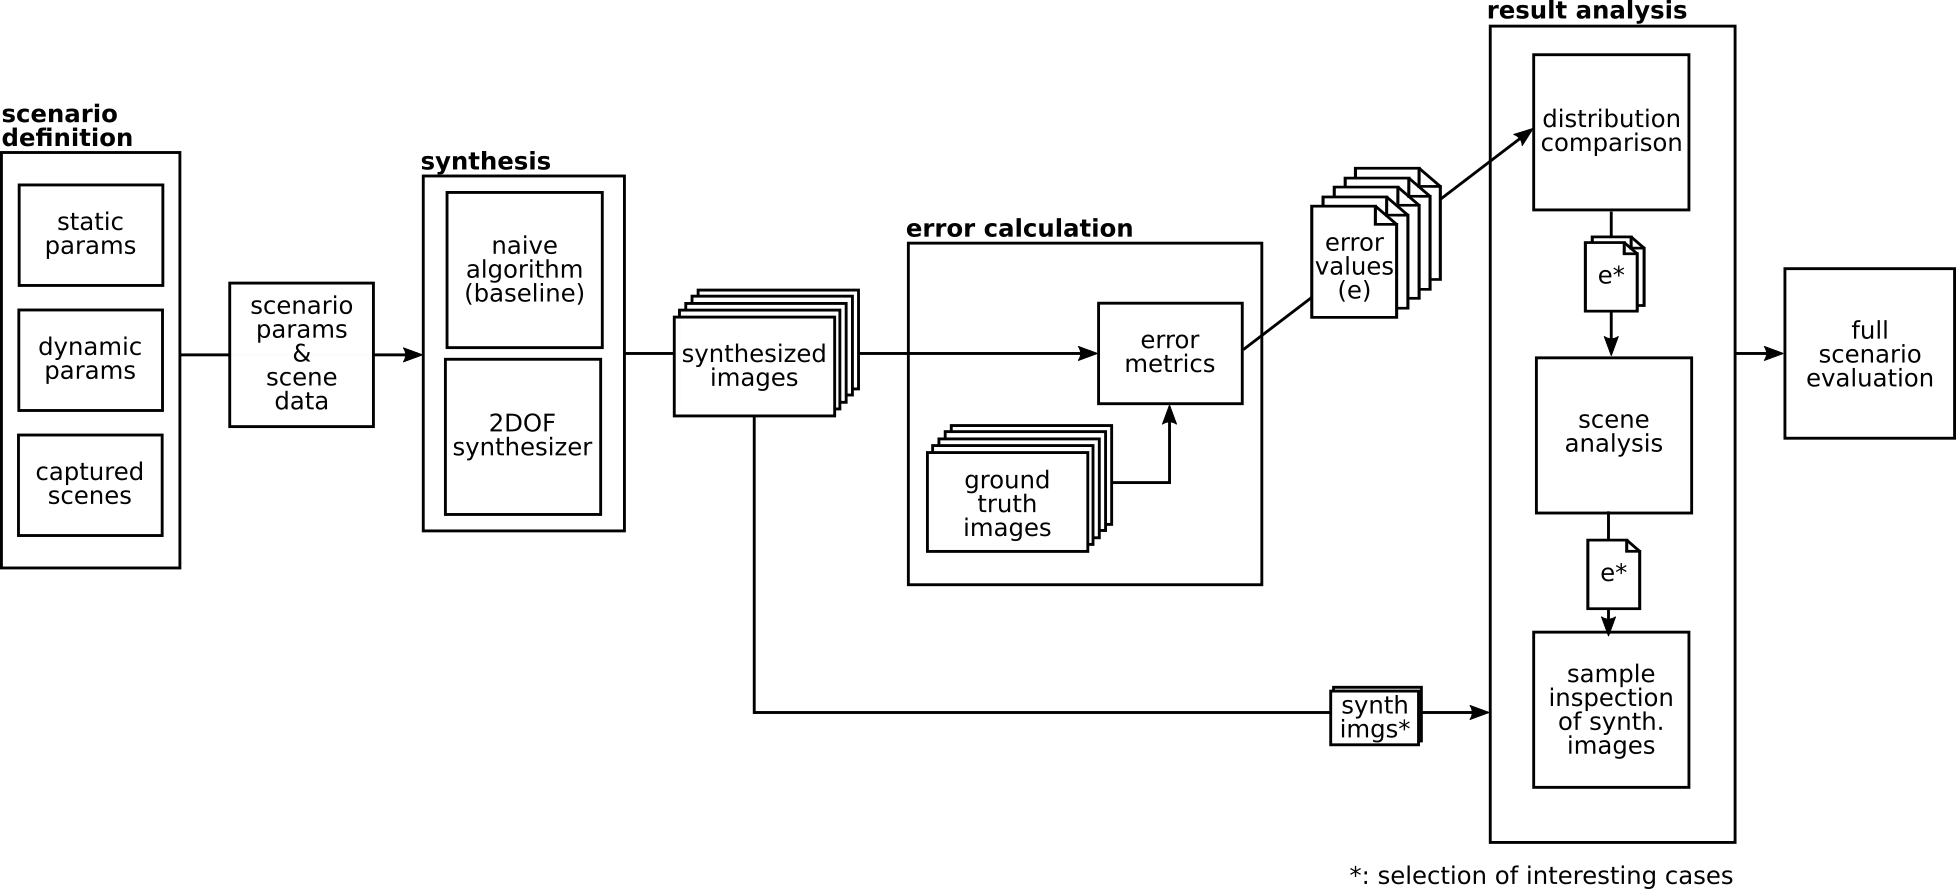
\includegraphics[width=\textwidth]{04/eval_methodology.png}
		\caption{Methodology for the evaluation of a scenario}
		\label{fig:eval-methodology}
\end{figure}

\subsubsection{Scenario Definition}
A scenario is defined by the parameter that it tests, the static parameters that are used, and the scene where the data was captured. Although a scenario is designed to test a specific parameter, which then is ``dynamic'' (i.e.\ will be modified throughout the scenario), there might also be more dynamic parameters. For example, in a scenario for exploring viewpoint density, the blending type might also be modified to see what effect the viewpoint density has on regular and flow-based blending. The static parameters include for example the location of the synthesized viewpoints, or any other parameter that remains unchanged throughout the scenario. One other defining factor of a scenario is the scene data that the scenario is tested on. Although the scene is part of the parameters (the external parameters, to be exact), it merits particular mention, as it contains the actual image data that is used for synthesis. This data, along with the other parameters defined in the scenario, are then passed on to the synthesis step.

%First, a scenario must be defined that illustrates the parameter that should be examined. This includes determining which of the parameters should be static, and which should be dynamic. There are two dynamic parameters at maximum, one to be examined, and one to increase the significance of the results. Adding more dynamic parameters per scenario would allow for a more definitive evaluation, but is outside of the scope of this thesis.

%The set of parameters (whether static or dynamic) contains the choice of scene in which to synthesize the images. The scene is defined by its captured viewpoints, metadata, and radius, which are all passed on to the synthesis step along with the other parameters defined for the scenario.

\subsubsection{Synthesis}
The synthesis step consists of two parts: the 2~DoF synthesis presented in Chapter~\ref{chap:implementation} using either flow-based blending or regular blending depending on the scenario parameters, and a baseline synthesis using a na\"ive algorithm.
The na\"ive algorithm consists of simply selecting the nearest neighbor viewpoint based on euclidean distance. The input parameters are the same for both algorithms and both results are passed on to error calculation.
The results of the na\"ive algorithm serve as a baseline comparison to verify whether the developed 2~DoF algorithm is an improvement to a na\"ive approach. If either the regular or the flow-based blending generally performed worse than the na\"ive algorithm, this would be an indication of a substantial flaw in the approach.

\subsubsection{Error Calculation}
There are many properties that a synthesis algorithm can be evaluated for, for example performance, visual acceptability (based on user studies), number of artefacts, or distance from the ground truth. In this evaluation, mathematical
%In order to evaluate the synthesized images, it is necessary to define metrics with which to measure their accuracy. Since it is outside of the scope of this thesis to evaluate the quality of the results based on human perception, mathematical
error metrics are used to compare each result to its ground truth image.  Two different metrics are chosen based on different image features so that potential limitations of each metric can be compensated for by the other. However, it must be taken into account that neither are perfect for the task of measuring accuracy on 360\degree synthesized images, so their validity should always be taken with a grain of salt. 

\paragraph{L1 error on RGB}
The first metric is the L1 error calculated on the ground truth and result images in RGB color space. This is a simple error metric that calculates the mean absolute difference of the RGB values and therefore indicates the mean accuracy of each pixel of the image. The RGB errors of each pixel are added together for the complete image and then divided by the number of pixels in the image. This results in an error value $e \in [0,3]$, since the maximum error per pixel is 3 for floating point RGB color values $\in [0,1]$.

The L1 error can also be visualized by calculating the absolute difference per pixel without averaging the values. Figure~\ref{fig:l1_example} shows an example visualization of the L1 error between two images. The visualization encodes areas of the image where there is a very large difference with a value closer to white and areas where there is no difference as black, which clearly highlights areas of the image that are problematic.

The L1 error is useful because it gives a rough estimation of how accurately each pixel is synthesized. The visualization indicates in which areas the synthesized image is inaccurate, which is helpful for classifying problems. However, a drawback of the L1 error is that it relies on color values, which means that images with large differences in pixel values will generally produce a higher error value than images with smaller differences in pixel values, even though the distortion and displacement may be the same.

\begin{figure}
\centering
    \hfill
    \begin{subfigure}[t]{0.3\textwidth}
            \centering
            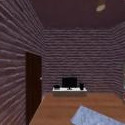
\includegraphics[width=0.9\textwidth]{04/l1_ex01.jpg}
            \caption{}
    \end{subfigure}%
    \hfill
    \begin{subfigure}[t]{0.3\textwidth}
            \centering
            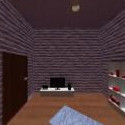
\includegraphics[width=0.9\textwidth]{04/l1_ex02.jpg}
            \caption{}
    \end{subfigure}
    \hfill
    \begin{subfigure}[t]{0.3\textwidth}
            \centering
            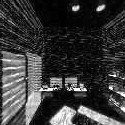
\includegraphics[width=0.9\textwidth]{04/l1_ex03.jpg}
            \caption{L1 error visualization of (a) and (b)}
    \end{subfigure}%
    \hfill
    \hfill
  \caption[Example visualization of L1 RGB error]{Example visualization of L1 RGB error. The RGB error values have been intensified so that they are more visible.} \label{fig:l1_example}
\end{figure}

As in the case of optical flow calculation, some adjustment must be made to adapt this metric for 360\degree images. Since the equirectangular projection is not equal-area, the areas towards the poles would intrinsically have higher weighting, since RGB L1 is calculated per pixel. To avoid this problem, the cube map projection is used, since it does not significantly distort the image. The average value is then calculated using the six faces of the cube, omitting the black background.

\paragraph{SSIM error on Grayscale}
The metric to complement the RGB L1 error is a variation of the the structural similarity index (SSIM) \cite{ssim}, which measures the \emph{structural similarity} between two images. Instead of comparing the images pixel by pixel, the SSIM uses the luminance, contrast and structure of the images for comparison. It compares these locally, i.e.\ it operates on smaller areas instead of the image as a whole. As a result, it is possible that the SSIM does not register small displacements in the scene if the objects are not distorted. However, the additional comparison with the RGB L1 error should mitigate this potential problem.

The SSIM metric in general, and the implementation used in the evaluation\footnote{skimage.metrics.structural\_similarity \cite{skimage}} return a value $\in [-1, 1]$ with 1 signifying an extremely similar image and -1 signifying a very different image. In order to more easily compare it with the RGB L1 error, the SSIM value is converted to an error value $ e \in [0,1]$, with 0 signifying an identical image (0 error) and 1 signifying a very different image.

The SSIM error is calculated on the grayscale image in cubemap representation. There is no need to use an RGB image, since it does not use the color values of an image. To avoid possible problems with distortion, the cubemap representation is again used.

\subsubsection{Result Analysis}
For each scenario evaluation, the number of results is made up of the dynamic parameters, the number of synthesized viewpoints, plus the baseline results. For each image, there are two error metrics to be considered.
%The number of parameters combined with the comparison to the baseline results and the use of two different error metrics results in a large number of error values.
In order to analyze these results effectively, it is necessary to break them down by creating different visualizations that highlight different attributes of the results.At first, an overview is created, from which interesting cases are selected and examined in more detail.

\paragraph{Distribution Comparison}
The first step of the analysis is a comparison of error value distribution. In order to compare all the error values of a scenario, they are plotted using a boxplot (Figure~\ref{fig:boxplot_example}). The different parameter combinations of the scenario are plotted on the y axis (e.g. viewpoint densities a, b, c) and the error distribution (i.e.\ the error values of all the synthesized viewpoints) is plotted on the x axis. The box plot shows the distribution of these values: the thick black line in the colored box is the median value (approx. 0.184 in Figure~\ref{fig:boxplot_example}), the colored ranges to the left and right of the median describe the ``interquartile range'' (IQR), the range of the closest half of the data (25\% on each side). The ``whiskers'' of the plot extend to the minimum and maximum of the values. The minimum and maximum are defined as $1.5\cdot IQR$. Any data outside of the the range between the minimum and the maximum, are the ``outliers'', depicted as small crosses. The boxplot gives a general overview of how the error values of the specific scene are distrubute. The distribution of the error values of the results in Figure~\ref{fig:boxplot_example}, for example, shows that the first three quartiles of the results are fairly close to the median (between approx. 0.14 and 0.19), whereas the fourth quartile extends, over almost the same range (0.19 to 0.225) and there are some extreme outliers. This indicates that there are some viewpoints that performed significantly worse than most of the others.

\paragraph{Scene Analysis}
Based on the insights gained in the distribution comparison, several interesting cases are selected for closer analysis. These cases are examined by color coding the error values and assigning the colors to the positions in the scene. This puts the error values in context with the scene surroundings. Figure~\ref{fig:posmap_example} shows the synthesized points in the context of the scene, color coded by their error values. The maximum and minimum values of the points (also clearly visible in Figure~\ref{fig:boxplot_example}) are coded as light green and dark blue, respectively. This visualization gives a more detailed overview over the values of the different points. In Figure~\ref{fig:posmap_example}, for example, the synthesized points near the right wall of the room have much better values than the row on the left side of the room. The four light green values are clearly the outliers that were visible in Figure~\ref{fig:boxplot_example}. Using this information, it is possible to draw som conclusions about the effect of the position of the synthesized viewpoint relative to the objects in the scene, and select a few synthesized images that merit closer examination.

\begin{figure}
\centering
    \hfill
    \begin{subfigure}[c]{0.5\textwidth}
            \centering
            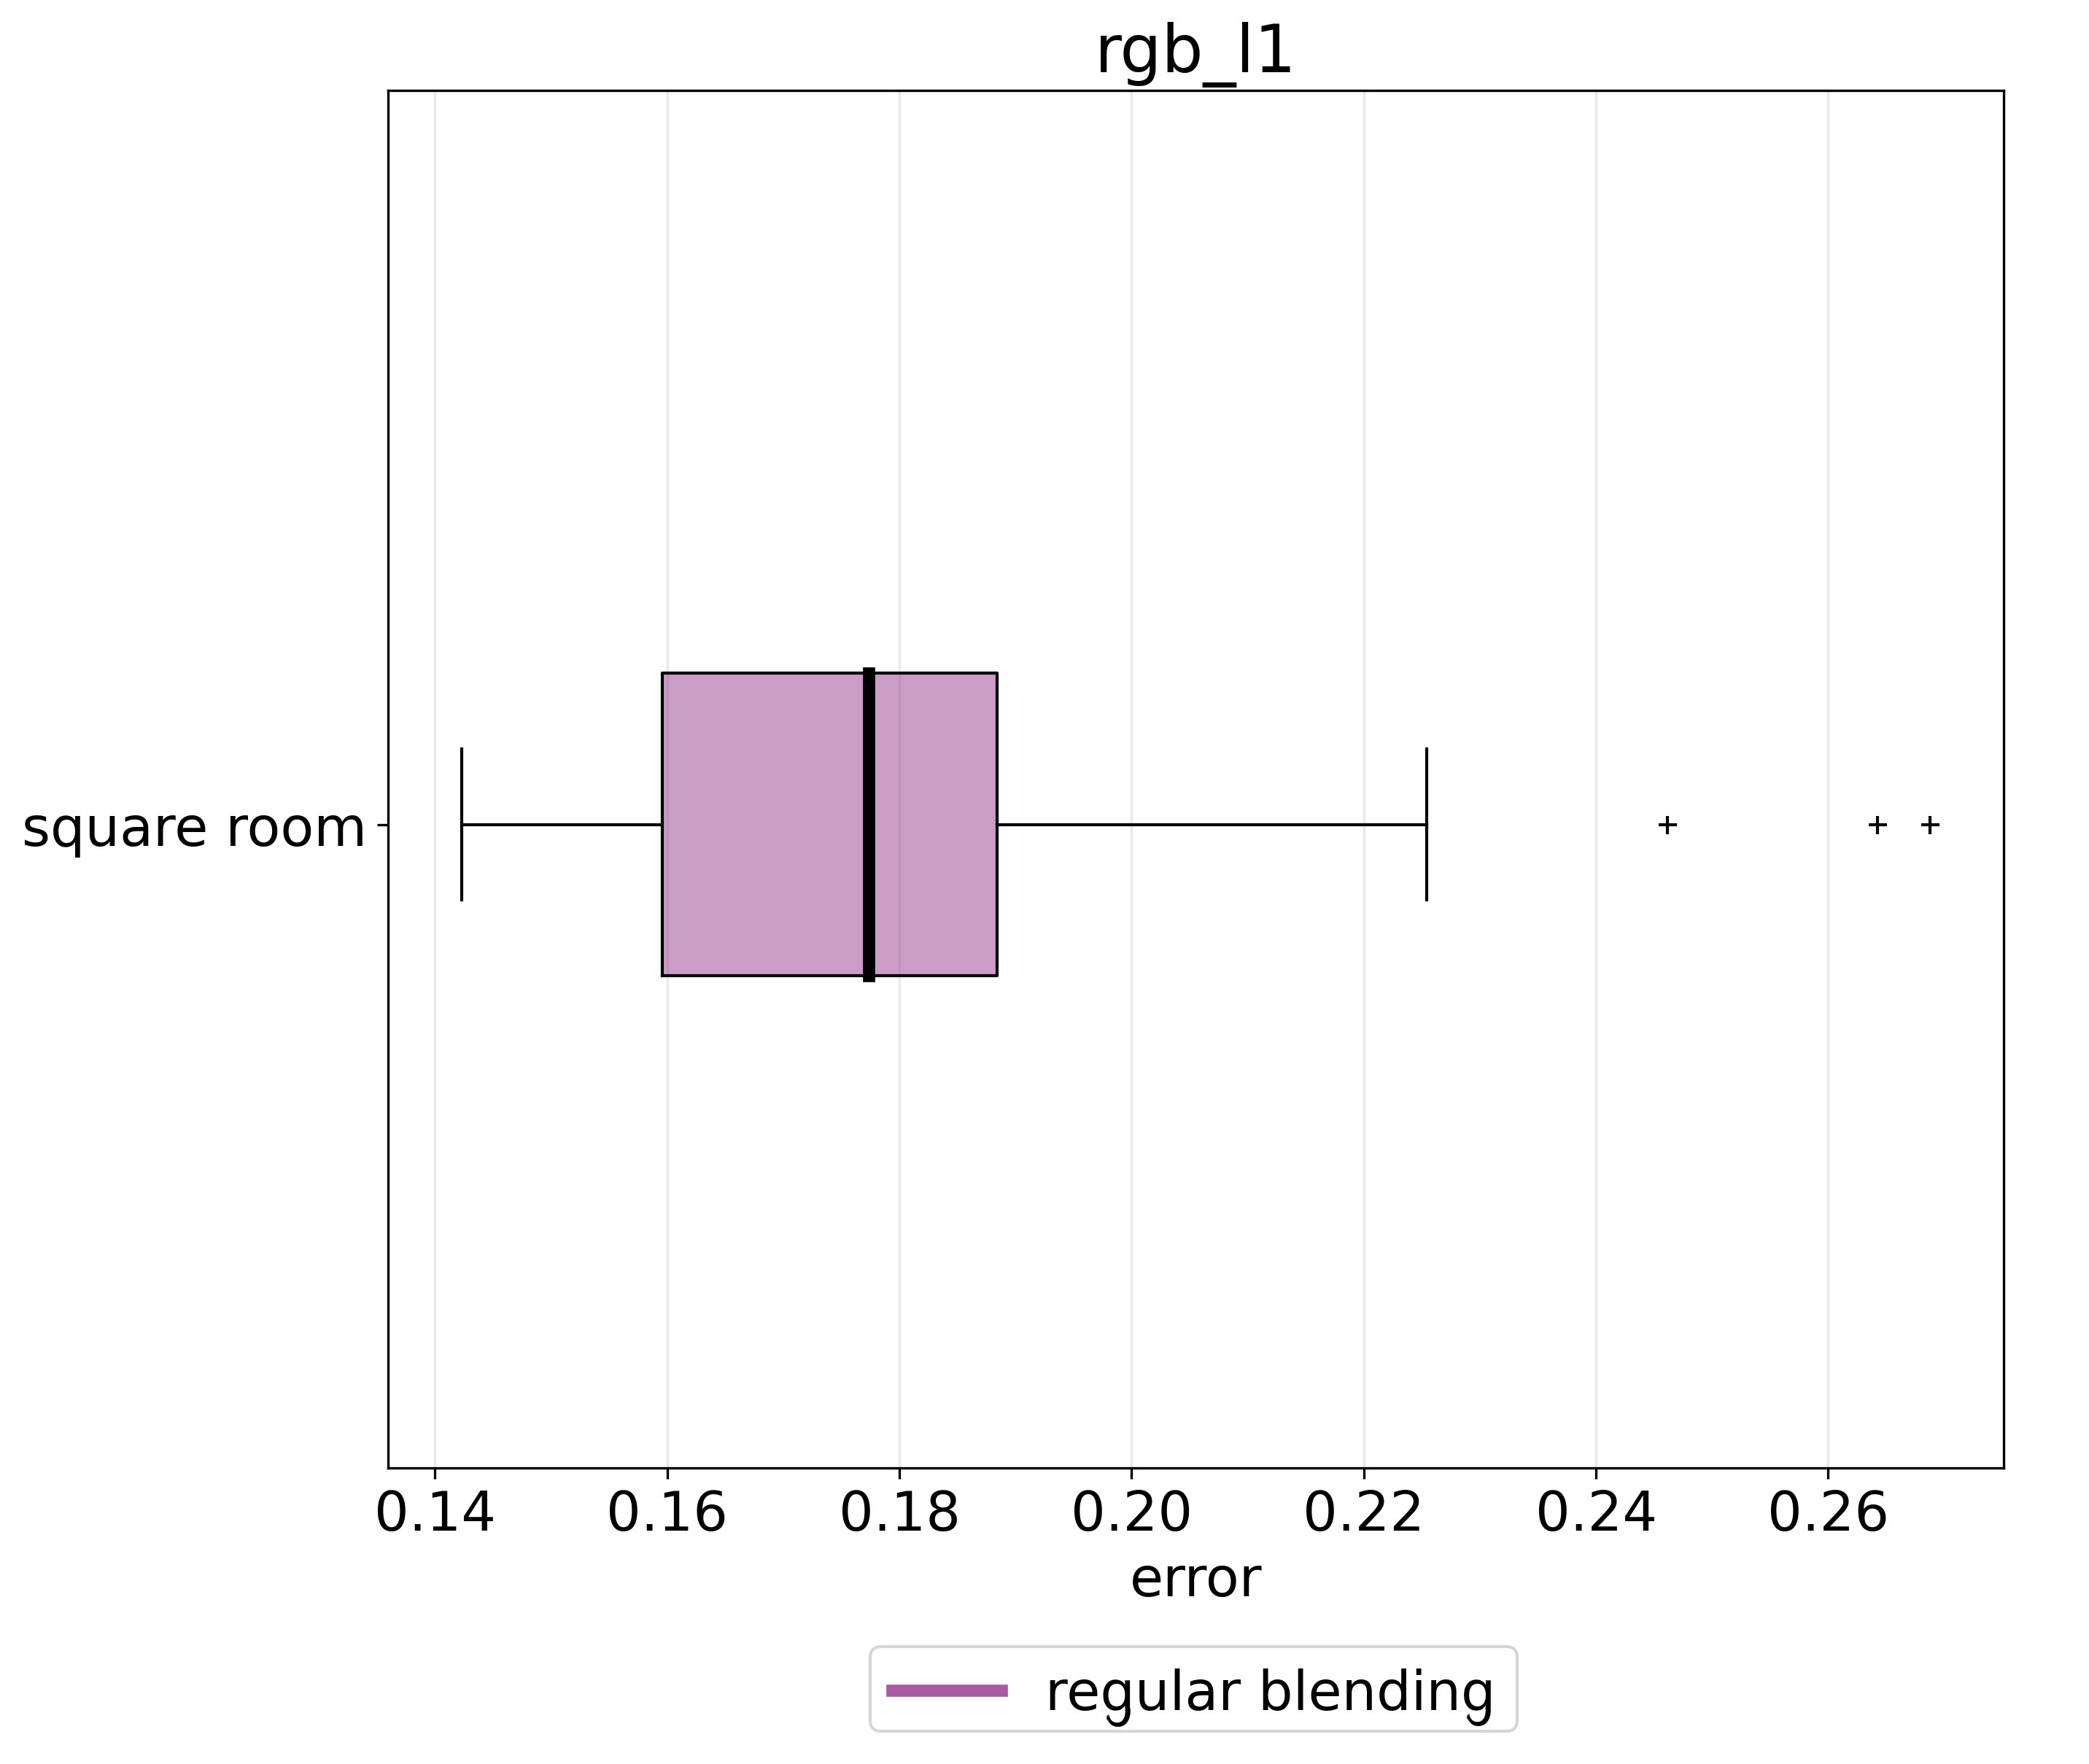
\includegraphics[height=6cm]{04/boxplot_example.jpg}
            \caption{Boxplot example for distribution comparison of the results of regular blending in the ``square room''} \label{fig:boxplot_example}
    \end{subfigure}%
    \hfill
    \begin{subfigure}[c]{0.5\textwidth}
            \centering
            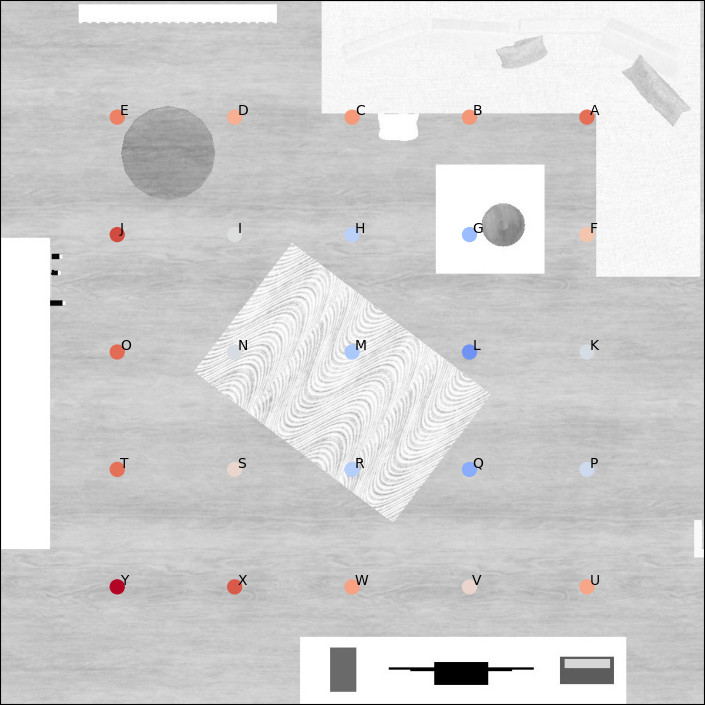
\includegraphics[height=6cm]{04/posmap_example.png}
            \caption{Visualization for scene analysis: The error values from the boxplot in (a) are mapped to colors at the positions of the viewpoints in the scene. Light green represents the worst value (approx. 0.27) and dark blue the best value (approx. 0.145).} \label{fig:posmap_example}
    \end{subfigure}
    \hfill
  \caption[Different types of result visualizations for L1 error values]{Different types of result visualizations for L1 error values (``rgb\_l1'') for example results of regular blending in a scene}
\end{figure}
\todo{replace figures (colors and error metric names}

\paragraph{Sample Inspection}
In order to further understand the effects of the parameters on specific positions, some of the synthesized viewpoints from the scene analysis are examined manually by comparing the synthesized image to the ground truth image. The visual examination may also reveal information that the error metrics are unable to extract, such as specific types of artefacts. For example, by using the information presented in Figure~\ref{fig:posmap_example}, it is possible to choose one of the best results, for example synthesized point ``K'' near the right wall in the middle. The close inspection of the synthesized images is shown in Figure~\ref{fig:inspection_example} (page~\pageref{fig:inspection_example} in Appendix~\ref{imgs}\footnotemark): In the left column from top to bottom are the ground truth image, the synthesized image using regular blending, and the synthesized image using flow-based blending. In the right column are the L1 difference images to the ground truth image. They can help with understanding the error values. For example, the rug in the bottom face (green ring) is improved in the flow result compared to the regular result in Figure~\ref{fig:inspection_example}. However, the flow result also has a fairly large artefact at the top of the door in the left face (magenta ring), which is not the case in the regular result. The green rings show improvements, and the magenta rings show artefacts or other problems.\todo{color coding of marks?}
\footnotetext{The synthesized images are shown in Appendix~\ref{imgs}, in order to avoid interrupting the flow of the text, since they take up a fairly large amount of space.}















\section{Evaluation using Virtual Scenes} \label{sec:limit_eval}
In the first part of the evaluation, virtual scenes are used to evaluate the effect of a chosen set of internal and external parameters on the accuracy of the results of the 2~DoF synthesis.
Virtual scenes allow full control over the external parameters, for example the scene geometry, and the positions of the captured viewpoints, as well as being less error prone than manual capture, where positional and rotational inaccuracies may be introduced. This also 
\todo{eek}
As a result, virtual scenes make it possible to test setups that would be unfeasible for real scenes, for example using a large number of captured viewpoints at varying locations in different scenes.
Additionally, since the evaluation is based on comparing the synthesized images to the ground truth, it is necessary to capture the ground truth images, along with the input viewpoints.
As a result, the scenarios can be designed independent of the constraints of the manual capture of real scenes.
%this limit evaluation is performed on virtual scenes created with the open source 3D animation software Blender \cite{blender}.
%The first step of the evaluation is to test the parameters of choice in a way that explores a large range of \ldots cases. 
The parameters that will be explored in the scenarios are:
\begin{itemize}
  \item proxy-scene difference (how dissimilar is the scene geometry from the proxy sphere geometry, including the objects within the scene)
  \item density of the captured viewpoints
  \item position of the synthesized points relative to the captured points
%  \item flow-based blending compared to regular blending
\end{itemize}

A scenario is designed for each of the three parameters, containing several different setups that are meant to test the limitations of the algorithm developed in Section~\ref{chap:implementation}. 

%Another factor that will be considered in all of the scenarios is the impact of the proximity and complexity of objects within the scene. However, since this is hard to parametrize, it will not be measured or explicitly tested.

%There is one internal parameter that is not specifically tested, but needs to be addressed, since it has a significant effect on the outcome of the flow-based blending: the optical flow algorithm. Fortunately, using virtual scenes generated with Blender can help mitigate mitigate this problem, since Blender has the capabilities to retrieve movement vectors from the geometry data, which can be used as optical flow.

\subsection{Data Acquisition and Featured Scenes} \label{subsec:data_acquisition}
%In order to be able to test these scenarios, it is necessary to generate appropriate scenes. However, the manual capture of viewpoints as well as ground truth data can be very time-consuming. Furthermore, since locations need to be recorded either by hand, or calculated by a structure-from-motion algorithm or something similar, it is possible that the final locations are not perfectly accurate. In order to circumvent these problems, virtual scenes are used for the evaluation of limits. 


Three different scenes were modeled for testing, using the animation software Blender \cite{blender}: the \emph{checkersphere}, the \emph{square room} and the \emph{oblong room}.% and the \emph{oblong room II}.

\paragraph{Checkersphere}
The \emph{checkersphere} (Figure~\ref{fig:checkersphere}) is a perfect sphere with a diameter of approximately 2m. Its surface is covered with a checkerboard pattern with alternating colors of dark blue, dark red, and dark green. It represents a scene where the geometry of the scene is exactly the same as the proxy geometry. Although this kind of room is not likely to exist in reality, it serves as a good baseline, since the result of the reprojection should be very close to the ground truth. The checkerboard pattern was chosen so that distortions or inaccuracies are more visible.


\paragraph{Square Room}
The \emph{square room} (Figure~\ref{fig:square_room}) is a room whose basic shape is a perfect cube with a side length of 3.5m. It contains an assortment of furniture\footnotemark: In one corner, there is an orange, L-shaped couch with dark blue and white cushions and a white marble coffee table with a dark blue bowl on it, and several small, simple black and white pictures on the wall behind the couch. There is a blue and white rug in the middle of the room, and to the left of the couch are a round blue table, as well as a white radiator. On the wall next to the blue table is a white marble bookshelf containing several red books, as well as three wine bottles, and two decorational objects in green and purple. Across from the couch is a low marble cabinet with a black monitor, a black laptop and a black speaker on it. To the left of the cabinet is a wooden door with a gray handle. The walls are brick, painted a dark purple and there is a lamp with a white lampshade hanging from the middle of the ceiling.

\footnotetext{The furniture models used in the square room and the oblong room are adapted from \url{https://www.cgtrader.com/free-3d-models/interior/living-room/low-poly-interior-57731178-c955-4625-9e44-109c8eea5ee2}, by user ``miha29076'', and the textures are adapted from \url{https://www.poliigon.com/texture/plaster-17}, \url{ https://www.poliigon.com/texture/fabric-denim-003}, \url{https://www.poliigon.com/texture/wood-fine-dark-004}, and \url{https://www.poliigon.com/texture/interior-design-rug-starry-night-001}. \emph{All accessed last on September 23, 2020}}

The intention of using the square room is to allow approximate accuracy for the reprojection step, while at the same time offering a more realistic indoor setting.

\paragraph{Oblong room}
The \emph{oblong room} (Figure~\ref{fig:oblong_room}) has a room size of approximately 5.5m x 3.5m and contains the same basic elements as the square room. It has the exact same furniture layout as the square room, except that some objects 

%The \emph{oblong room} (Figure~\ref{fig:oblong_room}) has a room size of approximately 5.5m x 3.5m and contains the same basic elements as the square room. There are two variations: the oblong room I, which has the exact same furniture layout as the square room, and the oblong room II, in which the furniture layout is modified. This modification can help in examining possible correlations of the scene geometry with the result. For example, the bookshelf is a fairly complex geometry that is at eye-level (as opposed to many other objects which are below eye-level). Placing it at different positions in the two scenes makes the correlation between the proximity to the bookshelf and the possibly worse results easier to recognize.

\begin{figure}[p]
\centering
    \hfill
    \begin{subfigure}[t]{0.7\textwidth}
            \centering
            \includegraphics[height=5cm]{04/checkersphere_overview.jpg}
            \caption{Latlong image from the center of the sphere}
    \end{subfigure}%
    \hfill
    \begin{subfigure}[t]{0.3\textwidth}
            \centering
            \includegraphics[height=5cm]{04/checkersphere_outside.jpg}
            \caption{View from the outside for reference}
    \end{subfigure}
    \hfill
  \caption{Overview of the ``checkersphere''}
  \label{fig:checkersphere}
\end{figure}

\begin{figure}[p]
\centering
    \hfill
    \begin{subfigure}[b]{0.7\textwidth}
            \centering
            \includegraphics[height=5cm]{04/square_overview.jpg}
            \caption{Latlong image from the center of the room}
    \end{subfigure}%
    \hfill
    \begin{subfigure}[b]{0.3\textwidth}
            \centering
            \includegraphics[height=5cm]{04/square_top.jpg}
            \caption{Top view}
    \end{subfigure}
    \hfill
  \caption{Overview of the ``square room''}
  \label{fig:square_room}
\end{figure}

\begin{figure}[p]
\centering
    \hfill
    \begin{subfigure}[b]{0.7\textwidth}
            \centering
            \includegraphics[height=5cm]{04/oblong_overview.jpg}
            \caption{Latlong image from the center of the room}
    \end{subfigure}%
    \hfill
    \begin{subfigure}[b]{0.3\textwidth}
            \centering
            \includegraphics[width=5cm]{04/oblong_top.jpg}
            \caption{Top view}
    \end{subfigure}
    \hfill
  \caption{Overview of the ``oblong room''}
  \label{fig:oblong_room}
\end{figure}

\begin{figure}
\centering
    \hfill
    \begin{subfigure}[b]{0.4\textwidth}
            \centering
            \includegraphics[width=0.9\textwidth]{04/vps_checkersphere.jpg}
            \caption{The captured viewpoints in the checkersphere}
    \end{subfigure}
    \hfill
    \begin{subfigure}[b]{0.4\textwidth}
            \centering
            \includegraphics[width=0.9\textwidth]{04/vps_square.jpg}
            \caption{The captured viewpoints in the square room}
    \end{subfigure}
    \hfill
    \hfill

    \hfill
    \begin{subfigure}[b]{0.4\textwidth}
            \centering
            \includegraphics[width=0.9\textwidth]{04/vps_oblong.jpg}
            \caption{The captured viewpoints in the oblong room}
    \end{subfigure}
    \hfill
    \hfill
  \caption[The grid of captured viewpoints in each scene, including the proxy geometry]{The grid of captured viewpoints in each scene, including the proxy geometry (not to scale)} \label{fig:vps_grid}
\end{figure}

\paragraph{}
Given the different scenes, it is necessary to choose comparable viewpoints to capture that will be used as input for the synthesis. Since the scenes all have similar scale, the viewpoint layout was chosen to be identical in all of the scenes. This means that all scenes contain 36 captured viewpoints, aligned in a regular grid of 6x6 viewpoints, with 60cm spacing. The grid of viewpoints is centered within the scene. This means that in the checkersphere (Figure~\ref{fig:vps_grid}a) and the square room (Figure~\ref{fig:vps_grid}b), the viewpoints cover approximately the complete scene, and in the oblong room, there is about a 1m area on each side of the grid that is not captured (Figure~\ref{fig:vps_grid}c and Figure~\ref{fig:vps_grid}d). It is necessary to take this difference in viewpoint coverage into account for the evaluation, since the viewpoints in the oblong room have a larger distance to two of the walls, which may have an effect on the accuracy of the results.

Since Blender is designed for creating animated movies, and not the capture of static viewpoints, some adjustments had to be made to be able to capture the chosen viewpoints (as well as the ground truth images): After choosing the positions of the input viewpoints for the scenes, the position of the camera for each captured viewpoint was stored as a keyframe, so that the batch of viewpoints could be rendered like an animation. In order to automatically assign the viewpoints and the ground truth points to the keyframes, and write out the metadata, a blender script was implemented. This way the locations of the viewpoints would always be perfectly accurate, and the ``capture'' of the viewpoints required no manual effort. The images were rendered with a resolution of 1000x500 for all of the scenes, in order to reduce the computation time for the image synthesis in the tests.


%, and the same number of synthesized viewpoints (25). Figure~\ref{fig:scene_setup} show how the points are set up in the different scenes. Using the same distances between viewpoints is important for comparing the accuracy (since larger distances may have an impact on the optical flow result), so the space occupied by the viewpoints is proportionally smaller in the oblong rooms (i.e. the viewpoints are not distributed in the entire room). This must be considered when evaluating the results.

\subsection{Synthesizing Ground Truth Optical Flow} \label{subsec:gt_of}
Using Blender to create virtual scenes not only facilitates capture, but also offers an alternative to calculating optical flow. As mentioned in Section~\ref{subsec:optical_flow}, most optical flow algorithms struggle with large displacements. The flow-based blending step in the 2~DoF synthesis algorithm, on the other hand, assumes decent optical flow and there is no attempt to judge whether the optical flow calculation is feasible between two selected viewpoints. As a result, given the wrong circumstances (two viewpoints A and B that are far apart), the optical flow algorithm may fail, leading the flow-based blending to output undesirable results. The success of the optical flow algorithm is a prerequisite for the success of the 2~DoF algorithm with flow-based blending.

However, the focus of this evaluation is not the accuracy of an arbitrary optical flow algorithm. In the best case, it would be possible to emulate ``perfect'' optical flow, thus decoupling the success of the optical flow from the success of the flow-based blending. While this is practically impossible for real scenes, virtual scenes theoretically contain all necessary information for retrieving ``ground truth'' optical flow. Blender, for example, is capable of ``rendering'' motion vectors using its vector speed render pass, which calculates the movement between points from one frame to the next in pixel space. The result is a motion vector field, which corresponds to the result of a ``classic'' optical flow algorithm. This, in the best case, ``ground truth'' optical flow was first presented by Butler et al.\ \cite{sintel} as a benchmark for optical flow algorithms.

In order to demonstrate the improvement of Blender optical flow compared to Farneb\"ack optical flow, which is the optical flow algorithm used in the implementation, Figure~\ref{fig:of_comparison}a shows a scene setup in which 25 viewpoints (A-Y) are synthesized using Farneb\"ack and Blender optical flow at the interpolation distance $\delta = 0.5$ between captured points. 
Figure~\ref{fig:of_comparison}b shows the improvement of the results using Blender optical flow: In all but one case for the L1 values, and in the majority of the SSIM values the Blender optical flow improved the error values. The visual difference of the 1~DoF interpolation is clear: Figure~\ref{fig:of_comparison}c shows the viewpoint ``I'' interpolated using Farneb\"ack optical flow, and Figure~\ref{fig:of_comparison}d the same viewpoint using Blender optical flow. There are distincly fewer artefacts with Blender optical flow, for example the rug and the couch both have a much more distinct outline, and the bookshelf is also clearer. Figure~\ref{fig:of_comparison}e and Figure~\ref{fig:of_comparison}f show the same for interpolated viewpoint ``M''. In this case, the TV cabinet and the rug are much clearer in the Blender optical flow version (Figure~\ref{fig:of_comparison}f).

\begin{figure}
\centering
    \hfill
    \begin{subfigure}[b]{0.4\textwidth}
            \centering
            \includegraphics[width=0.9\textwidth]{04/gt_flow/1DoF_scene.png}
            \caption{The viewpoints for testing optical flow}
    \end{subfigure}
    \hfill
    \begin{subfigure}[b]{0.4\textwidth}
            \centering
            \includegraphics[width=0.9\textwidth]{04/gt_flow/blender_flow_improvement_small.png}
            \caption{The improvement of error values using Blender optical flow vs Farneb\"ack optical flow}
    \end{subfigure}
    \hfill
    \hfill
\par\bigskip
    \hfill
    \begin{subfigure}[b]{0.4\textwidth}
            \centering
            \includegraphics[width=0.9\textwidth]{04/gt_flow/I_calcflow.jpg}
            \caption{1~DoF interpolated viewpoint ``I'' using Farneb\"ack optical flow}
    \end{subfigure}
    \hfill
    \begin{subfigure}[b]{0.4\textwidth}
            \centering
            \includegraphics[width=0.9\textwidth]{04/gt_flow/I_blenderflow.jpg}
            \caption{1~DoF interpolated viewpoint ``I'' using Blender optical flow}
    \end{subfigure}
    \hfill
    \hfill
\par\bigskip
    \hfill
    \begin{subfigure}[b]{0.4\textwidth}
            \centering
            \includegraphics[width=0.9\textwidth]{04/gt_flow/M_calcflow.jpg}
            \caption{1~DoF interpolated viewpoint ``M'' using Farneb\"ack optical flow}
    \end{subfigure}
    \hfill
    \begin{subfigure}[b]{0.4\textwidth}
            \centering
            \includegraphics[width=0.9\textwidth]{04/gt_flow/M_blenderflow.jpg}
            \caption{1~DoF interpolated viewpoint ``M'' using Blender optical flow}
    \end{subfigure}
    \hfill
    \hfill
  \caption{Comparing 1~DoF interpolation results using Farneb\"ack to results using Blender optical flow} \label{fig:of_comparison}
\end{figure}

%\begin{figure}
%		\centering
%		\includegraphics[width=\textwidth]{04/blender_flow_improvement.png}
%		\caption[Accuracy improvement with Blender flow versus Farneb\"ack flow]{Accuracy improvement with Blender flow versus Farneb\"ack flow: The y axis shows the improvement of the error metric when using Blender flow.}
%		\label{fig:calc_vs_synth_flow}
%\end{figure}

It is notable that using Blender's optical flow tends to improve the results, compared to Farneb\"ack's algorithm, but that does not mean that the resulting optical flow is necessarily accurate. For example, the bookshelf in the right and middle faces in Figure~\ref{fig:of_comparison}d still shows warping and doubling effects, indicating that there are still some inaccuracies. The same is true for the coffee table and the blue round table in the bottom face. There are several possible reasons for this, mostly based on the fact that the process in Blender, like most optical flow algorithms, is designed for frame-to-frame use, and has in this case been ``misused'' for distances that are infeasible for an actual animation. Nevertheless, no definitive explanation can be made at this point, since this would require in-depth understanding of Blender's vector speed render pass, which is outside of the scope of this thesis. Based on the results shown in Figure~\ref{fig:of_comparison}, and experience gained from testing both variants, the Blender optical flow is used for the limit evaluation, because, even though it is not perfect, it still seems to mostly yield better results than Scipy's implementation of Farneb\"ack's optical flow algorithm and as such decouples (to a degree) the success of the 2~DoF synthesis with flow-based blending from the success of the optical flow algorithm.

%\begin{itemize}
%   \item points that are not visible because of perspective shift will not have a correspondence
%   \item distortion due to wide fov may have an effect on the results
%   \item even blender motion vectors are for frame to frame use, so it is possible, that large jumps do not work well because the blender algo can't handle it
%\end{itemize}

\subsection{Scenarios and Results}
Using the generated scenes and optical flow, as well as the parameters defined for this evaluation, it is now possible to design, test, and evaluate the following scenarios:
\begin{itemize}
  \item ``Different Scene Geometries''
  \item ``Density of Captured Viewpoints''
  \item ``Position of Synthesized Viewpoints Relative to Captured Viewpoints''
\end{itemize}

This section presents the scenes, viewpoint setups, and tested parameters used in each of these scenarios, as well as the results of the tests, which are evaluated using distribution comparison, scene analysis, and sample inspection, as described in Section~\ref{sec:eval_methodology}. First the effect of the tested parameter on the regular blending results is examined, then the effect on the flow-based blending results is examined, and finally, the the results of the flow-based blending are compared to the results of the regular blending.

\subsubsection{Different Scene Geometries}
The first parameter to be examined is the effect of different scenes on the accuracy of the results. There are two attributes of a scene that may have an influence on the result: the basic shape of the scene (e.g. sphere, cube, rectangular prism, or arbitrary polygon), and the objects within the scene. All the scenes presented in \ref{subsec:data_acquisition} are used, as they differ both in their basic shape, as well as in the arrangement of the objects within, although the square room and the oblong room are more similar to each other than to the checkersphere.
%A key factor of this scenario is how different the scenes are from the proxy geometry. The larger the difference, the more inaccurate the result of the reprojection will be.

The arrangement of captured viewpoints in all the scenes is identical (a 6x6 grid with a spacing of 60cm), and 25 viewpoints are synthesized in each scene (Figure~\ref{fig:scene_setup}). The synthesized points are near or in the center of each grid cell, since these are the areas where the deviation angles are the highest, and where the largest artefacts for the regular blending are expected to emerge. In the square and oblong rooms, the synthesized points are slightly offset from the center of each grid cell (Figure~\ref{fig:scene_setup}). The offset is important in order to test actual 2~DoF synthesis, instead of just 1~DoF interpolation, since synthesizing in the center of a grid cell could be done with only 1~DoF interpolation (e.g. by interpolating by 0.5 between the top right to the bottom left captured viewpoint, as was done in Section~\ref{subsec:gt_of} for testing Blender optical flow). No offset was used in the checkersphere scene, since the checkersphere scene is expected to have excellent results for the regular blending (since the proxy geometry and scene geometry are identical). In this case it is more interesting to use one of the presumably best positions for the flow-based blending to see how well it holds up in comparison.

\begin{figure}
\centering
    \hfill
    \begin{subfigure}[b]{0.4\textwidth}
            \centering
            \includegraphics[width=\textwidth]{04/scenario_scene/sphere_points.jpg}
            \caption{The checkersphere}
    \end{subfigure}%
    \hfill
    \begin{subfigure}[b]{0.4\textwidth}
            \centering
            \includegraphics[width=\textwidth]{04/scenario_scene/square_points.jpg}
            \caption{The square room}
    \end{subfigure}
    \hfill
    \hfill

    \hfill
    \begin{subfigure}[b]{0.4\textwidth}
            \centering
            \includegraphics[width=\textwidth]{04/scenario_scene/oblong_points.jpg}
            \caption{The oblong room}
    \end{subfigure}%
    \hfill
%    \begin{subfigure}[b]{0.4\textwidth}
%            \centering
%            \includegraphics[width=\textwidth]{04/scenario_scene/oblong2_points.jpg}
%            \caption{The oblong room II}
%    \end{subfigure}
%    \hfill
    \hfill
  \caption[The captured and synthesized viewpoints in the different scenes]{The captured (blue) and synthesized (orange) viewpoints in the different scenes (scenes are not to scale)} \label{fig:scene_setup}
\end{figure}

\begin{figure}
\centering
    \hfill
    \begin{subfigure}[b]{0.45\textwidth}
            \centering
            \includegraphics[width=\textwidth]{04/scenario_scene/boxplot_regular.png}
            \caption{Regular blending}
    \end{subfigure}
    \hfill
    \begin{subfigure}[b]{0.45\textwidth}
            \centering
            \includegraphics[width=\textwidth]{04/scenario_scene/boxplot_flow.png}
            \caption{Flow-based blending}
    \end{subfigure}
    \hfill
  \caption{Comparing the distributions of the results in different scenes}
  \label{fig:scene_boxplot_split}
\end{figure}

\paragraph{Regular Blending Results}
Figure~\ref{fig:scene_boxplot_split}a shows the distributions of the error values for the regular blending results in the three scenes. The most striking feature of this distribution is that the checkersphere results show the highest error values for the L1 error, whereas they show the lowest values for the SSIM error. At first, this seems surprising, both because the error metrics do not ``agree'', as well as because the results of the regular blending are expected to be very good since the scene geometry is identical to the proxy geometry. The reason for the ambiguous results is the sensitivity of the L1 metric to different color values. L1 errors on the RGB images of the checkersphere will produce a higher value in general because of the checkerboard texture:
The difference between a dark blue pixel of a dark checkerboard field, and a white pixel on a white checkerboard field is close to 1, whereas the difference between a dark brown pixel and a dark purple pixel (e.g. between the door and the wall in one of the rooms) will produce a lower error value, although the distortion or displacement may be identical. The SSIM error metric, which does not take the color values of the pixels into account, produces a distribution that is much closer to the expected result: Since the scene geometry is identical to the proxy geometry, the result of the reprojection should be almost perfect. And in fact, when visually comparing the results of a synthesized viewpoint to the ground truth (Figure~\ref{fig:scene_checkersphere_Y}, page~\pageref{fig:scene_checkersphere_Y}), the only difference is a little bit of blurriness due to sampling differences. The L1 difference depicted in the right column of Figure~\ref{fig:scene_checkersphere_Y} shows how the blurriness caused the high L1 error.

The trend of the error metrics of the other two rooms is consistent: Both the L1 and SSIM error values of the square room are generally higher than those of the oblong room. In this case, comparing the RGB color values is more reliant, since both rooms use the same textures. The results however, are surprising: Although the basic geometry of the square room is closer to the proxy geometry, the error values from the square room are generally higher than those from the oblong room.
A closer scene analysis (Figure~\ref{fig:scene_regular_square_oblong}) shows the probable reason for this: The error values in the square room (Figure~\ref{fig:scene_regular_square_oblong}a) are particularly high near the bookshelf on the left side of the room. Comparing the synthesized images at location ``O'' (right in front of the bookshelf) for the two scenes (Figure~\ref{fig:scene_O_regular}, page~\pageref{fig:scene_O_regular}) confirms this impression: The bookshelf is so close to viewpoint ``O'' in the square room, that there are extreme inaccuracies in the synthesis due to large deviation angles. In the oblong room, the bookshelf is much further away, making the devation angles much smaller and the result more accurate. The larger net distance to the walls and some of the objects in the oblong room is the likely reason for the lower error results throughout the scene.

\begin{figure}
\centering
    \hfill
    \begin{subfigure}[b]{0.45\textwidth}
            \centering
            \includegraphics[width=\textwidth]{04/scenario_scene/01_square__regular.png}
            \caption{Results of regular blending in the square room}
    \end{subfigure}
    \hfill
    \begin{subfigure}[b]{0.45\textwidth}
            \centering
            \includegraphics[width=\textwidth]{04/scenario_scene/01_oblong__regular.png}
            \caption{Results of regular blending in the oblong room}
    \end{subfigure}
    \hfill
  \caption{Scene analysis of regular blending results in the square and oblong rooms} \label{fig:scene_regular_square_oblong}
\end{figure}

\paragraph{Flow-based Blending Results}
The distribution of error values of the synthesis using flow-based blending in the different scenes (Figure~\ref{fig:scene_boxplot_split}b) show similar tendencies as the error values of the regular blending, in that the L1 values of the checkersphere are very high, and the results of the oblong room generally have lower values than those of the square room. One exception is the SSIM error value of the checkersphere: Where the SSIM error in the checkersphere scene is significantly lower than the other two for the regular blending results, in the flow-based blending results, the SSIM error yields worse results than the oblong room, but still mostly better than the square room. The worse performance of the flow-based blending in the checkersphere is likely due to the fact that the flow-based blending introduces some inaccuracies, for example due to imperfect optical flow, or ray approximation. Figure~\ref{fig:scene_checkersphere_Y} (page~\pageref{fig:scene_checkersphere_Y}) shows slightly higher inaccuracies for the flow result, as well as some artefacts and noise, that are the likeliest causes for the higher error values.

In the other cases, the results of the flow-based blending mirror those of the regular blending: The error values in the oblong room are generally lower than those in the square room. Looking at the example viewpoint ``O'' in Figure~\ref{fig:scene_O_flow} (page~\pageref{fig:scene_O_flow}) shows that, like in the case of the regular blending, this is due to the relative postion of the walls and objects to the points: like the regular blending, the flow-based blending also performs a lot worse when there is a detailed object in close proximity. In the case of the regular blending, the reason for this are the large deviation angles leading to inaccurate reprojections. Generally, the flow-based blending should improve this problem, however, in this case it did not (or not considerably), which is mostly due to the optical flow calculation failing in proximity to the bookshelf, which was demonstrated in Section~\ref{subsec:gt_of}. If the optical flow algorithm does not produce accurate results, the flow-based blending will not, either.
The result in the square room in Figure~\ref{fig:scene_O_flow} clearly shows the effect of the failed optical flow on the synthesized image. The normally straight lines of the books are warped (marked in magenta), but a comparison to the ground truth shows that they are warped in a way that bears no resemblance to the actual position or shape.

\paragraph{Comparing Regular Blending to Flow-based Blending Results}

\begin{figure}
		\centering
		\includegraphics[width=\textwidth]{04/scenario_scene/all_boxplot.png}
		\caption[The distribution of results in different scenes]{Comparing the distribution of the results in different scenes for the na\"ive algorithm, regular blending, and flow-based blending}
		\label{fig:scenario_scene_boxplot}
\end{figure}

The distributions of the error values of both the regular blending (purple) and the flow-based blending (blue) are shown in Figure~\ref{fig:scenario_scene_boxplot}, as well as the error value distribution of the na\"ive algorithm (orange) for comparison\footnotemark. The graph shows that the error values of the results of the flow-based blending are generally slightly better than those of the regular blending (except in the case of the checkersphere) and that the error values of the results of the regular blending tend to be distinctly better than those of the na\"ive algorithm. 
\footnotetext{The na\"ive algorithm error values of the checkersphere were omitted because they were so much higher than the other values that the scale of the plot became too small.}

In the case of the checkersphere, where the scene geometry is identical to the proxy geometry, the regular blending distinctly outperforms the flow-based blending. However, this is to be expected. The goal of the flow-based blending approach aims to improve problems that arise due to the difference between the real and proxy geometries, and it introduces possible inaccuracies (viewpoint selection, optical flow, ray approximation) in order to do so. Therefore, it is not surprising that the results are less accurate than the results of the regular blending.

For the square room and the oblong room, the $\Delta L1$ and $\Delta SSIM$ of the flow-based blending versus the regular blending are shown in Figure~\ref{fig:scene_diff_square_oblong}. Positive $\Delta L1$ and $\Delta SSIM$ values (red) signify that the flow-based blending produced a \emph{worse} result than the regular blending, and negative $\Delta L1$ and $\Delta SSIM$ (blue) signify that the flow-based blending produced a \emph{better} result than the regular blending, with stars marking the highest and lowest values. At a glance, it is clear that in all cases in the oblong room, and in all but one or two cases in the square room (depending on the metric) the flow-based blending improves the result based on the L1 and SSIM error metrics. However, the L1 value range is larger in the oblong room than it is in the square room (max. improvement of 0.037, compared to 0.015 in the square room), which most likely indicates more visible improvements in the oblong room.

Figure~\ref{fig:scene_square_N} (page~\pageref{fig:scene_square_N}) shows the viewpoint with the lowest (best improved) $\Delta L1$ difference in the square scene. The most visible difference is the rug on the bottom face: In the regular blending result, it shows some ghosting (doubled, offset edges), which has been mostly fixed in the flow-blending result. Other than that, the white coffee table with the blue bowl in the left face is slightly blurrier, but covers a more accurate area than the result of the regular blending, and the bottom part of the bookshelf is more accurate. Otherwise the two results are very similar visually.
For the ``worst improved'' viewpoint L (Figure~\ref{fig:scene_square_L}, page~\pageref{fig:scene_square_L}) the regular and flow results are also visually very similar. The most visible differences are that the rug shows some ghosting artefacts in the regular blending result, which are gone in the flow-based result. However, the flow-based blending introduced some new artefacts, namely a sharp discontinuity and offset on the rug, and a distorted edge on the coffee table.
%are that the rug in the left face of the flow result is more accurate than in the regular result. On the other hand, the flow result shows black lines on the right face which are due to a bug in one of the libraries. Since the increase of the L1 and SSIM errors are extremely small, this may in part be due to the implementation problems discussed in Section~\ref{subsec:bugs}.

Figure~\ref{fig:scene_oblong_A} (page~\pageref{fig:scene_oblong_A}) shows viewpoint ``A'' with the best improvement in the oblong scene. Here, the most visible difference is the couch in the left and bottom faces. Where the inner edge of the couch shows severe ghosting artefacts in the regular image, it is much cleaner in the flow-based result. The rug also covers a more accurate area of the image. However, the flow-based blending also introduces new artefacts, for example in the bottom face, where a part of orange couch appears detached from the rest of the couch.
The ``worst improved'' viewpoint L (Figure~\ref{fig:scene_oblong_L}) shows even more of these artefacts: The rug in the bottom face has a few extreme discontinuities, as well as the coffee table in the left face (although the coffee table is positioned more accurately in the flow-based blending result). The severe discontinuities are caused by the selection of input viewpoints for flow-based blending: For each ray of the synthesized image, two input viewpoints are selected based on their deviation angle, and whether they are ``on either side'' of the ray in question (see Section~\ref{subsec:2dof_flow-based}). This means that while traversing the rays of synthesized viewpoint there comes a point where the selected input viewpoints for the 1~DoF interpolation A and B suddenly switch to B and C (this will be described in more detail in Section~\ref{subsec:discussion_virtual}). In these cases, the less accurate the reprojection step is, the more extreme the discontinuity at that place in the image seems to be. Although these discontinuities are visually extremely irritating, it is possible that they do not have a large impact on the error metrics.

\begin{figure}
\centering
    \hfill
    \begin{subfigure}[b]{0.45\textwidth}
            \centering
            \includegraphics[width=\textwidth]{04/scenario_scene/diff_square_regular-flow.png}
            \caption{Square room}
    \end{subfigure}
    \hfill
    \begin{subfigure}[b]{0.45\textwidth}
            \centering
            \includegraphics[width=\textwidth]{04/scenario_scene/diff_oblong_regular-flow.png}
            \caption{Oblong room}
    \end{subfigure}
    \hfill
  \caption[Improvement of flow-based blending results over regular blending results in the square and oblong rooms]{$\Delta L1$ and $\Delta SSIM$, ``improvement'' of flow-based blending over regular blending results in the square and oblong rooms. The stars denote the best and worst cases.} \label{fig:scene_diff_square_oblong}
\end{figure}

\paragraph{Scenario Synopsis}
The goal of this scenario was to evaluate the effects of the scene geometry on the accuracy of the results of regular and flow-based blending. This includes the details of the geometry given by the shape and placement of objects within the scene, as well as the general shape of the scene.
Concerning the geometry details, i.e. the objects within the scene, the results of the scenario are fairly clear: both blending techniques perform better, the further away specific objects are from the synthesized point. The closer the synthesized point gets to an object, the more ghosting and doubling artefacts and positional inaccuracies show up in the regular blending results. In some of these cases, the flow-based blending synthesizes a more accurate image, showing fewer positional inaccuracies and correctly synthsizing some of the object shapes. However, the flow-based blending also introduced some new artefacts, predominantly abrupt discontinuities. These discontinuities were not necessarily recognized by the error metrics and needed to be identified by visual inspection. In the case of extreme proximity to an object (e.g. in front of the bookshelf), both the regular blending and the flow-based blending produced highly inaccurate results. In the case of the flow-based blending, this was due to inaccurate optical flow. However, even though the optical flow was inaccurate, the flow-based blending result was not worse (in terms of the error metrics) than the regular blending result.
%Given the three input scenes, as well as the captured viewpoints and the locations of the synthesized viewpoints in this scenario, the measured results indicate that for scenes where the proxy geometry is identical to the scene geometry, the regular results have very low L1 and SSIM error values, whereas using flow-based blending increases the error value. For the scenes where the proxy geometry differs from the real scene geometry, in the majority of tested cases, the flow-based blending produced better results.

As for the impact of the general shape, the results are not very significant, due to the choice of the oblong and square rooms along with the chosen captured and synthesized viewpoints. The different distances of the objects to the synthesized viewpoints within the two scenes overpowered most effects that the different basic shape might have had. It was clear, however, that in the case where the scene geometry matched the proxy geometry, the flow-based blending performed worse than the regular blending.

%In summary, the results of the synthesis in the three different scenes indicate that, unsurprisingly, the general shape of the scene has an impact on the accuracy of the results: The results of the checkersphere are visually extremely accurate for regular blending, and mostly accurate for flow-based blending. However, the impact of the general shape seems to have a much smaller influence compared to the impact of the details of the geometry and the proximity of complex objects to the synthesized viewpoint. This is especially clear when comparing the results of the square and the oblong room. Although the general shape of the square room is closer to the proxy sphere, the results in the oblong room are better, due to the larger net distance of the viewpoints to the objects. This is the case for both regular and flow-based blending.






















\subsubsection{Density of the Captured Viewpoints}
The previous scenario demonstrated that close proximity of a synthesized viewpoint to an object can have a strong adverse effect on the accuracy of the result. A possible way to mitigate this problem could be to increase the density of the captured viewpoints near objects. The scenario presented in this section explores the impact of viewpoint density on the accuracy of the results.

To test the effect of viewpoint density, the square room is used, as the viewpoint grid covers the entire area of the room, which guarantees higher proximity to all the objects. Three different versions of the captured viewpoint grid are used: a 2x2 grid with a spacing of approximately 2.3m (Figure~\ref{fig:density_setup}a), the 6x6 grid with a spacing of approximately 60cm, as was used in the previous scenario (Figure~\ref{fig:density_setup}b), and a 12x12 grid with a spacing of approximately 30cm (Figure~\ref{fig:density_setup}c). The 2x2 grid was chosen since it is the minimal grid to cover the entire room, and the 12x12 grid was chosen, since it halves the distance of the 6x6 grid and as such, retains the relative position of the captured viewpoints compared to the synthesized viewpoints. If a different grid was used, for example 10x10, some synthesized viewpoints would be closer to captured viewpoints than other synthesized viewpoints, which may have an effect on the overall results.
Like in the previous scenario, 25 viewpoints are synthesized, located near the center of each grid cell. They are offset slightly from the exact center, like in the previous scenario, to demonstrate true 2~DoF synthesis.

\begin{figure}
\centering
    \hfill
    \begin{subfigure}[t]{0.3\textwidth}
            \centering
            \includegraphics[width=\textwidth]{04/scenario_density/2x2_points.jpg}
            \caption{A density of 4 viewpoints (2x2 grid)}
    \end{subfigure}
    \hfill
    \begin{subfigure}[t]{0.3\textwidth}
            \centering
            \includegraphics[width=\textwidth]{04/scenario_density/6x6_points.jpg}
            \caption{A density of 36 viewpoints (6x6 grid)}
    \end{subfigure}
    \hfill
    \begin{subfigure}[t]{0.3\textwidth}
            \centering
            \includegraphics[width=\textwidth]{04/scenario_density/12x12_points.jpg}
            \caption{A density of 144 viewpoints (12x12 grid)}
    \end{subfigure}
    \hfill
  \caption[The different captured viewpoint densities in the square room]{The different captured viewpoint densities (blue) in the square room with the synthesized viewpoints (orange)} \label{fig:density_setup}
\end{figure}

\begin{figure}
\centering
    \hfill
    \begin{subfigure}[b]{0.5\textwidth}
            \centering
            \includegraphics[width=\textwidth]{04/scenario_density/boxplot_regular.png}
            \caption{Regular blending}
    \end{subfigure}%
    \hfill
    \begin{subfigure}[b]{0.5\textwidth}
            \centering
            \includegraphics[width=\textwidth]{04/scenario_density/boxplot_flow.png}
            \caption{Flow-based blending}
    \end{subfigure}
    \hfill
  \caption[Comparing the distributions of the results with different densities separately]{Comparing the distributions of the results in the square room with different densities separately}
  \label{fig:density_boxplot_split}
\end{figure}

\paragraph{Regular Blending Results}
Figure~\ref{fig:density_boxplot_split}a shows the general distribution of the results of the regular blending with varying viewpoint densities. Unsurprisingly, the accuracy of the results improves, the higher the density of the input viewpoints is.
In the 6x6 and the 12x12 setup, there are several outliers with a higher error value for the L1 error, which are likely due to the proximity of some points to the bookshelf. In the 2x2 setup, there are no significant outliers, possibly because the error values are more uniform throughout the scene.

A look at the scene visualization in Figure~\ref{fig:density_regular_scene_analysis} confirms these assumptions: The outliers in the 6x6 and 12x12 setups are caused by the bookshelf on the left side of the room. In the case of the 2x2 setup, the error values are fairly high throughout, compared to the other two setups, which is the reason that the viewpoints near the bookshelf do not register as outliers. Other than the area around the bookshelf, both the 6x6 and the 12x12 scenes have a fairly uniform distribution for the L1 error. For the SSIM error, the areas close to the walls have a slightly higher error than those in the middle of the scene. This is in line with the results of the previous scenario, where the error values near objects or walls tended to be higher.

Although the error values near objects and walls are slightly higher in both the 6x6 and 12x12 setups, the improvement when going from the 6x6 to the 12x12 density is also higher in these areas, as can be seen in Figure~\ref{fig:dens_diff_6x6_12x12}a. This figure shows the improvement when using the 12x12 scene versus the 6x6 scene. In areas near walls (e.g. the top row for both metrics, viewpoints A-E), or objects (in front of the bookshelf for L1, viewpoints O and T, or in front of the TV screen for L1 and SSIM, viewpoints U,V,W), the improvement tends to be higher than near the center of the scene (e.g. viewpoints H, G, M, L).

In order to understand more about how the density affects ghosting and other artefacts in the images, one of the better and one of the worse results for all of the setups is examined visually. According to the general tendencies of the values in the different setups (Figure~\ref{fig:density_regular_scene_analysis}), synthesized viewpoint ``T'' near the bottom left of the room, next to the bookshelf has a comparatively high error value in both metrics for all three scenes and synthesized viewpoint ``G'', above the coffee table towards the top right corner has a comparatively low error value for all of the scenes.
Figure~\ref{fig:density_regular_T} (page~\pageref{fig:density_regular_T}) shows why T has a high error value: for the 2x2 scene, while most of the scene is moderately accurate (the objects are in approximately the right place), the bookshelf is shown from the wrong perspective, i.e. from the side versus from the front. The reason for this is that the perspective of the bookshelf of the viewpoint used for reprojection was from the side. Using only this information, it is impossible to reconstruct the front of the bookshelf. One other effect of the fairly large jump in perspective using only regular blending are the warped walls. This is due to using the sphere as proxy geometry. The warping problems are much less visible in the 6x6 and 12x12 results, since the reprojection jumps are much smaller due to the captured viewpoints being much closer together. While the L1 difference images on the right do show an improvement of the accuracy in the 12x12 image over the 6x6 image, it is not as visually obvious in the result image as might be expected from halving the distance between the viewpoints. The bookshelf still has many inaccuracies due to its proximity and high detail.
However, while the difference between the 12x12 and the 6x6 image is not very evident in one of the worse results, Figure~\ref{fig:density_regular_G} (page~\pageref{fig:density_regular_G}) better illustrates the effect of the denser grid. The 2x2 image excellently demostrates the problem with using input images with large deviation angles in conjunction with a proxy geometry that is not identical to the scene geometry: The rays used to synthesize this image captured the coffee table at different positions and the reprojection does not account for this, since it only approximates the scene geometry by using the proxy geometry. As a result, the coffe table appears four times. In this example, the reprojection errors decrease visibly as the density increases: in the 6x6 image, a slight doubling effect of the coffe table is still visible, whereas in the 12x12 image, the table only appears slightly blurry.

\begin{figure}
\centering
    \hfill
    \begin{subfigure}[b]{0.32\textwidth}
            \centering
            \includegraphics[width=\textwidth]{04/scenario_density/01_2x2_regular.png}
            \caption{Results of regular blending with a 2x2 grid}
    \end{subfigure}
    \hfill
    \begin{subfigure}[b]{0.32\textwidth}
            \centering
            \includegraphics[width=\textwidth]{04/scenario_density/01_6x6_regular.png}
            \caption{Results of regular blending with a 6x6 grid}
    \end{subfigure}
    \hfill
    \begin{subfigure}[b]{0.32\textwidth}
            \centering
            \includegraphics[width=\textwidth]{04/scenario_density/01_12x12_regular.png}
            \caption{Results of regular blending with a 12x12 grid}
    \end{subfigure}
    \hfill
  \caption{Scene analysis of the regular blending results in the square room with different densities} \label{fig:density_regular_scene_analysis}
\end{figure}

\begin{figure}
\centering
    \hfill
    \begin{subfigure}[b]{0.45\textwidth}
            \centering
            \includegraphics[width=\textwidth]{04/scenario_density/diff_regular-regular.png}
            \caption{Improvement for regular blending}
    \end{subfigure}
    \hfill
    \begin{subfigure}[b]{0.45\textwidth}
            \centering
            \includegraphics[width=\textwidth]{04/scenario_density/diff_flow-flow.png}
            \caption{Improvement for flow-based blending}
    \end{subfigure}
    \hfill
  \caption{Improvement of results using 12x12 density compared to 6x6 density} \label{fig:dens_diff_6x6_12x12}
\end{figure}


\paragraph{Flow-based Blending Results}
%The error values of the flow-based blending results show similar tendencies as the regular blending results: The 6x6 and 12x12 setups have a few outliers, which can be attributed to the area near the bookshelf. The 2x2 
%The doubling effect visible in the regular results should be improved by using the flow-based blending, as long as the flow-based blending can accurately calculate optical flow. The farther apart the captured viewpoints are, the more likely this is to fail.
The error values of the flow-based blending results (Figure~\ref{fig:density_boxplot_split}) show similar tendencies as the regular blending results. Like for the regular blending, the 6x6 and 12x12 setups have several outliers in the L1 metric, but otherwise a fairly close distribution. The scene visualization (Figure~\ref{fig:density_flow_scene_analysis} also shows a similar pattern: In the 2x2 scene, the error values are generally high, whereas in the 6x6 and 12x12 scenes, the error values are high near the bookshelf, but generally similar everywhere else. Like in the regular blending scene, the improvement of the values in the 12x12 setup compared to the 6x6 setup is slightly higher near the walls. Since the tendencies are very similar as in the regular blending, it is more interesting to examine the comparison of the regular blending to the flow-based blending, instead of the flow-based blending by itself, as there do not seem to be any findings other than the improvement of the results with higher density, especially near the walls.

\begin{figure}
\centering
    \hfill
    \begin{subfigure}[b]{0.32\textwidth}
            \centering
            \includegraphics[width=\textwidth]{04/scenario_density/02_2x2_flow.png}
            \caption{Results of flow-based blending with a 2x2 grid}
    \end{subfigure}
    \hfill
    \begin{subfigure}[b]{0.32\textwidth}
            \centering
            \includegraphics[width=\textwidth]{04/scenario_density/02_6x6_flow.png}
            \caption{Results of flow-based blending with a 6x6 grid}
    \end{subfigure}
    \hfill
    \begin{subfigure}[b]{0.32\textwidth}
            \centering
            \includegraphics[width=\textwidth]{04/scenario_density/02_12x12_flow.png}
            \caption{Results of flow-based blending with a 12x12 grid}
    \end{subfigure}
    \hfill
  \caption{Scene analysis of the flow-based blending results in the square room with different densities} \label{fig:density_flow_scene_analysis}
\end{figure}


\paragraph{Comparing Regular Blending to Flow-based Blending Results}
The tendencies of the regular blending results compared to the flow-blending results shown in Figure~\ref{fig:scenario_dens_boxplot} are not immediately apparent. Only the results of the 6x6 scene show a consistent improvement of the flow-based results compared to the regular results. For the 2x2 scene, the median L1 error is higher for the flow-based blending, while the error range is lower. The SSIM error for the 2x2 scene, however, is clearly lower for the flow-based blending. In the 12x12 scene, the L1 error shows an almost identical distribution, whereas for the SSIM result, the general distribution of the flow-based blending is wider, which implies that some results were improved while others were worsened.

Figure~\ref{fig:dens_diff_2x2_12x12} shows the improvements of the flow-based blending over the regular blending for the 2x2 and the 12x12 scenes. Both the 2x2 and the 12x12 scenes show improved values nearer to the walls, and a slightly worse values near the center of the room. However, although this overview shows similar tendencies, a look into the synthesized images shows some of the fallacies of the metrics. 

For the 2x2 scene, the regular blending produced relatively inaccurate results, due to the extreme perspective changes. The flow-based blending relies on optical flow, which does not handle large displacements well (even with Blender optical flow). The results show that in the 2x2 scene, the optical flow algorithm did not produce very accurate results, which is visible in both the ``best'' and ``worst improvement''. Figure~\ref{fig:density_2x2_best_worst} (page~\pageref{fig:density_2x2_best_worst}) The ``best improvement'' image (Figure~\ref{fig:density_2x2_best_worst}a) is the image that was one of the worst rated for the regular blending, since it did not correctly show the bookshelf. In the flow-based version, a blurry shadow of the bookshelf is visible, however, the whole image shows blurry distortions of all of the objects. So although the metrics show an improved value, visually it is much harder to distinguish the different objects. The same holds true for the ``worst improvement'' image, where both metrics measured a slight increase in error value from the regular to the flow-based result. Figure~\ref{fig:density_2x2_best_worst}b shows point ``K'', and while the regular blending result shows extreme artefacts due to doubling, the flow-based version, due to the failure of optical flow, exacerbates the problem: some objects, such as the rug, are reduced to a blurry spot, whereas others, such as the coffee table, suffer from even worse blurring. In summary, it is safe to say that the captured viewpoints in the 2x2 density are too far apart to produce any satisfying results.

As for the 12x12 scene, The error metrics show a slight decrease in error values near the walls, and a slight increase of error values near the middle of the scene. However, when looking at the best and worst improvement in Figure~\ref{fig:density_12x12_best_worst} (page~\pageref{fig:density_12x12_best_worst}, very little difference is actually visible. In the best improvement image (Figure~\ref{fig:density_12x12_best_worst}a), the flow-based blending slightly improves the accuracy of the bookshelf in the right and back faces, although some ghosting artefacts remain. It also does not display an artefact present in the front face of the regular blending result (a white blurry spot, which appears due to the use of an input viewpoint that had a deviation angle of zero at that position, but seems to have captured a part of the bookshelf with that ray). However, other than that, the two images are visually extremely similar. The same holds true for the ``worst improvement'' (Figure~\ref{fig:density_12x12_best_worst}b): Looking at the L1 difference images, it is hard to see any difference between the two, but when comparing the synthesized images, it is noticeable that the flow-based blending removed the ghosting artefacts on the rug and the coffee table. This change is so slight that it is not surprising that it did not register with the metrics. Visually however, the flow-based blending result seems more accurate, since it improves the ghosting artefacts. An explanation for the lower rating by the SSIM metric could be that some of the straight lines that have ghosting artefacts in the regular blending result (e.g. the right edge of the coffee table) are rated higher than the same lines in the flow-based blending result, that do not display ghosting artefacts, but are slightly warped. Since the SSIM metric uses structural elements, it is possible that it prefers the version with the ghosting artefacts.

The 6x6 scene is more straightforward. Figure~\ref{fig:dens_diff_6x6} shows the improvement of the flow-based blending results over the regular blending results. As this is very similar to the improvement in the previous scenario for the square room (Figure~\ref{fig:scene_diff_square_oblong}a), where an improvement was achieved by the flow-based blending, the images are not examined in detail.

\begin{figure}
		\centering
		\includegraphics[width=\textwidth]{04/scenario_density/boxplot_all.png}
		\caption[Comparing the distributions of all of the results with different densities]{Comparing the distributions of the results in the square room with different densities of captured viewpoints for the regular blending and flow-based blending}
		\label{fig:scenario_dens_boxplot}
\end{figure}

\begin{figure}
\centering
    \hfill
    \begin{subfigure}[b]{0.45\textwidth}
            \centering
            \includegraphics[width=\textwidth]{04/scenario_density/diff_2x2_regular-flow.png}
            \caption{Improvement in the 2x2 scene}
    \end{subfigure}
    \hfill
    \begin{subfigure}[b]{0.45\textwidth}
            \centering
            \includegraphics[width=\textwidth]{04/scenario_density/diff_12x12_regular-flow.png}
            \caption{Improvement in the 12x12 scene}
    \end{subfigure}
    \hfill
  \caption[Improvement of flow-based blending results over regular blending results in the 2x2 and 12x12 scenes]{Improvement of flow-based blending results over regular blending results in the 2x2 and 12x12 scenes} \label{fig:dens_diff_2x2_12x12}
\end{figure}

\begin{figure}
		\centering
		\includegraphics[width=0.45\textwidth]{04/scenario_density/diff_6x6_regular-flow.png}
		\caption[]{Improvement of flow-based blending results over regular blending results in the 6x6 scene}
		\label{fig:dens_diff_6x6}
\end{figure}

\paragraph{}
In summary it can be said that for the tested room (and presumably in most other cases, as well), increasing the density of the captured viewpoints also increases the accuracy of the results. In the tested cases, the improvement was more apparent near objects and walls.

In the extreme case of the 2x2 density, both the regular and the flow-based blending lead to extreme artefacts, due to the large jumps in reprojection and the failure of the optical flow algorithm.
For the 6x6 density, the results are unambiguous: both metrics produce lower error values for the flow-based blending than for the regular blending.
sing the 12x12 density results in fairly low errors and few artefacts for both regular and flow-based blending. In this case, the metrics are ambiguous, since the difference between the two versions is very small. A visual evaluation of some of the samples indicates that the flow-based blending improves ghosting artefacts, which visually improves the images, even though the error metric may be slightly higher.















\subsubsection{Position of Synthesized Viewpoints Relative to Captured Viewpoints}
In most of the previous results, the flow-based blending showed an improvement over the regular blending. However, the locations of the synthesized viewpoints were chosen explicitly so that the regular blending would most likely have the most difficulty: areas near the center of the grid cells with comparably high deviation angles. Naturally, this is not the only location that comes in question for synthesis. In fact, all locations within the convex hull can potentially be synthesized by the 2~DoF algorithm. In order to gain a more general understanding of the impact of the relative positons of the captured viewpoints on regular versus flow-based blending, this scenario synthesizes a dense grid of viewpoints, instead of choosing a few select locations in the scene, like in the previous scenarios.

Based on the insights gained from the last two scenarios, the square room is used with a captured viewpoint density of 6x6. The square room gives the advantage of covering the whole possible space, and a density of 6x6 with a spacing of 60cm is a conceivable distance for extrapolation to real scenes. A grid of 25x25 viewpoints is synthesized, totaling 625 synthesized points (Figure~\ref{fig:scenario_offset_setup}).

\begin{figure}
		\centering
		\includegraphics[width=0.3\textwidth]{04/scenario_offset/dense_points.jpg}
		\caption[The dense grid of synthesized viewpoints in the square room]{The dense grid of synthesized viewpoints (orange) and the 6x6 grid of captured viewpoints (blue) in the square room}
		\label{fig:scenario_offset_setup}
\end{figure}

\paragraph{Regular Blending Results}
In this scenario, only the position of the viewpoints within a single scene is examined, so the distribution can be inspected directly in the scene analysis visualization (Figure~\ref{fig:offset_regular_flow}a). The dense coverage of synthesized viewpoints gives a fairly detailed picture of the effects of the location relative to the scene, and especially relative to the location of the captured viewpoints. It is immediately striking that the synthesized viewpoints in the close vicinity of a captured viewpoint have a distincly lower error value than viewpoints that are farther away. The exceptions to this are the synthesized viewpoints near the walls and near the bookshelf. The observation of higher error values near the bookshelf and walls are consistent with the observations in the previous scenarios. However, this scenario shows that the error values are higher near walls and objects, independent of whether the synthesized viewpoints are close to the captured viewpoints or not. This phenomenon is clearly visible in the L1 error visualization, but even more so in the SSIM error visualization, where the accuracy dropoff is even more extreme. 


\paragraph{Flow-based Blending Results}
The error values of the flow-based blending results (Figure~\ref{fig:offset_regular_flow}b) display a different pattern than those of the regular results: While the error values are lower in the vicinity of captured viewpoints, they are comparably low in the vertical and horizontal spaces between the captured viewpoints, as well. This implies that it does not make a big difference to the error values whether a synthesized viewpoint is very close to a captured viewpoint, or anywhere between a set of horizontally or vertically adjacent viewpoints. In general, the majority of the values is fairly similar, with clear outliers only visible near the bookshelf.

\begin{figure}
\centering
    \hfill
    \begin{subfigure}[b]{0.45\textwidth}
            \centering
            \includegraphics[width=\textwidth]{04/scenario_offset/01_analysis_regular.png}
            \caption{Results of regular blending}
    \end{subfigure}
    \hfill
    \begin{subfigure}[b]{0.45\textwidth}
            \centering
            \includegraphics[width=\textwidth]{04/scenario_offset/01_analysis_flow.png}
            \caption{Results of flow-based blending}
    \end{subfigure}
    \hfill
  \caption{Scene analysis of regular and flow-based blending results} \label{fig:offset_regular_flow}
\end{figure}

\paragraph{Comparing Regular Blending to Flow-based Blending Results}

\begin{figure}
		\centering
		\includegraphics[height=0.8\textheight]{04/scenario_offset/diff_square_regular-flow.png}
		\caption{Improvement of flow-based blending results over regular blending results for 625 synthesized images in the square room}
		\label{fig:scenario_offset_diff}
\end{figure}

%Just by inspecting the scene analysis visualization of the regular and flow-based blending results (Figure~\ref{fig:offset_regular_flow}) indicates that there are areas in which the regular blending performs better, and others in which the flow based blending does.
Figure~\ref{fig:scenario_offset_diff} shows the $\Delta$ L1 and SSIM error values when using the flow-based blending compared to the regular blending. Here, the results are clear: In general, the error values of synthesized points in close proximity to captured points go up (i.e. the accuracy gets worse) when using flow-based blending. An exception to this are the captured points near the walls of the room: In these cases, the flow-based blending improves the results in the majority of cases. Also, in the areas where the distance to the captured viewpoints is highest, the flow-based blending also performs better. An area where the results are ambiguous is the area near the bookshelf. Here, the improvement or degradation cannot be clearly attributed to the proximity to a captured viewpoint or the proximity of the bookshelf. It must be kept in mind, however, that in the case of the bookshelf, the Blender optical flow does not yield good, or even acceptable results, which has a direct, detrimental effect on the flow-based blending, so the results near the bookshelf should not be taken into strong consideration.

In many of the cases where the flow-based blending improves the result, it does so by shifting objects into more accurate positions. Figure~\ref{fig:offset_good}a shows one of these cases: The couch and the coffee table in the bottom face of the regular blending result are offset by a noticeable amount from the ground truth. The flow-based blending result shows almost no offset. It does introduce some new artefacts, for example blurriness and some discontinuities, which will be explained in Section~\ref{subsec:discussion_virtual}. Figure~\ref{fig:offset_good}b shows a similar example, where the rug in the bottom face shows a ghosting effect in the regular result, as well as being slightly offset from the ground truth position. Again, the flow-based result improves these errors, in this case only introducing a slight visual discontinuity.

In the areas close to captured viewpoints, where the flow based blending performs worse than the regular blending, a look at the images themselves is required to attempt to explain this unexpected result. Figure~\ref{fig:offset_bad}a shows an example where most of the image is very similar, except some distinctive artefacts in the bottom face (the blue table is misshapen) and in the left face (the coffee table displays a distinct edge and displacement). Figure~\ref{fig:offset_bad}b shows a different example, where the difference between the flow-based and the regular results is barely visible: There is a slight distortion at the top of the door in the left face, and the coffee table has a slightly larger offset.

Some of the artefacts in the flow-based blending results are undoubtedly due to the approach (e.g. ray approximation). However it is also possible that part of the reason for the higher error values for the flow-based blending results are part be due to the implementation problems discussed in Section~\ref{subsec:bugs}, since these only affect the flow-based blending and not the regular blending.


%l1 reg best:254 , worst:249
%ssim reg best: 254, worst: 572

%l1 flow best:475, worst: 274
%ssim flow best: 475, worst: 322
%with gt correction:
%l1 best: 475, 254, 279, worst: 274, 249, 299
%ssim best: 124,100,253, worst: 447, 322, 424

%worst improvement flow over reg:
  %l1: (inverse!) 478 504 270 373 496 520 395 246 272 145 120 424 370 245 371 349 271 396
  %ssim: (inverse!) 115 514 495 114 479 109 515 509 379 254 104 240 504 120 270 395 145 370 245 520
%best improvement flow over reg:
  %l1:52 72 567 552  67 569  62 442 444 427 302 593  57 319 445 581 177 223
  %ssim:52 72 552 567  93 569  57 598  67  62  98 562 554  70 593  43  28  60 

%average l1 improvement after correction: 0.123
%average ssim improvement after correction: 0.0790


%\begin{figure}
%		\centering
%		\includegraphics[width=0.6\textwidth]{04/scenario_offset/dense_boxplot.png}
%		\caption{Distribution of results for 625 points}
%		\label{fig:scenario_offset_boxplot}
%\end{figure}


\subsection{Discussion} \label{subsec:discussion_virtual}
The results of the 2~DoF synthesis with regular blending in the tested scenarios, were very much as expected. Areas where the proxy geometry deviated strongly from the actual geometry (e.g. near detailed objects) showed moderate to severe ghosting artefacts or displacements. Nonetheless, the results using regular blending generally had lower error values than the na\"ive algorithm, and in some cases, even than the flow-based blending.

In the majority of the tested cases, the flow-based blending produced lower error values than the regular blending. However, the evaluation also uncovered some factors that decreased the accuracy of the results, originating from the implementation details as well as the underlying approach:

\begin{itemize}
  \item failure of the optical flow algorithm
  \item bugs in external libraries
  \item deviation-angle-based choice of input viewpoints with abrupt change
  \item ray approximation
\end{itemize}

The failure of the optical flow algorithm, notably in the cases where a viewpoint was in close proximity to the bookshelf, presumably degraded the results of the flow-based blending considerably. However, since it was not possible to test with perfect optical flow, it remains unclear whether even ``perfect'' optical flow could improve the accuracy of viewpoints that are extremely close to objects, as there would still be large occluded areas. However, for areas where there is little occlusion, different optical flow algorithms may 

Furthermore, a factor that may have caused elevated error values is the due to reprojection problem in the external library Skylibs \cite{skylibs}. This bug, which leads to slight pixel offsets and thin black lines in the flow-based blending results, exclusively (as the regular blending does not use the problematic operation), may have a noticeable impact on the $\Delta$ L1 and SSIM error values in cases where the results are very similar. However, this error is very difficult to quantify, since the flow-based blending result contains strips of a number of 1~DoF interpolated images, which display the problem to varying degrees. As a result, it can only be assumed that this bug may have a noticeable impact on the decrease of accuracy in the flow-based blending results.

The accuracy of the optical flow, and the bug in the external library are both implementation-related problems, as they are not part of the approach. However, there are also some problems that are intrinsic to the approach and thus need to be discussed in more detail.

The most visible problem that is intrinsic to the approach is the choice of input viewpoints per pixel. This, in combination with the reprojection using the proxy geometry, is the reason for the abrupt jumps and discontinuities in the flow-based blending results. Figure~\ref{fig:flow_problem_oblong} breaks down the cause of the problem step-by-step: Looking at an arbitrary synthesized viewpoint in the oblong room (Figure~\ref{fig:flow_problem_oblong} that displays this problem, the abrupt discontinuities are clearly visible, for example in the rug in the bottom and right faces. 
In the synthesis process for each pixel of this image, two viewpoints A and B are chosen that are on either side of the ray corresponding to the pixel (Section~\ref{subsec:2dof_flow-based}). If more than one viewpoint is found on either side of the ray, the points with the smallest deviation angles are chosen. The interpolation distance between these points A and B is then calculated and the 1~DoF interpolation is performed. Finally the interpolated point is reprojected to the position of the synthesized viewpoint.
This succession of operations is performed for each ray of the synthesized image. As a result, there are areas in the synthesized image, where, from one pixel to the next, a different set of input viewpoints is chosen. This leads to image areas (``panels'') originating from a 1~DoF interpolation between different sets of input viewpoints (Figure~\ref{fig:flow_problem_oblong}b). When applying these panels to the synthesized image (Figure~\ref{fig:flow_problem_oblong}c), it becomes clear that these are the source of the abrupt continuities.
Figure~\ref{fig:flow_problem_oblong}d shows a visualization of the scene with an approximation of the rays that are associated with each panel\footnote{The rays were inserted by hand, so they are not 100\% accurate in terms of deviation angles}.

The switch between viewpoint sets within the image is not necessarily a problem in itself, given the 1~DoF interpolation worked well, and the reprojection was more or less accurate. However, in the cases where the proxy geometry deviates strongly from the actual geometry, the reprojection will introduce inaccuracies, which are exacerbated by the discontinuities.
%If, for example, only one interpolated image was calculated for the entire synthesized image, there would be no discontinuities. However, doing this would also remove the 
For example, the square room's geometry is closer to the proxy geometry. When comparing a very similar viewpoint from the square room with the example from the oblong room, (Figure~\ref{fig:flow_problem_square}), some discontinuities are hardly visible, for example at the coffee table, or on the door. Other discontinuities are visible, but less apparent since the displacement is relatively small, for example on the rug, or on the TV cabinet.

\begin{figure}
\centering
    \hfill
    \begin{subfigure}[c]{0.45\textwidth}
            \centering
            \includegraphics[width=\textwidth]{04/cubevis_result_extended_oblong.jpg}
            \caption{An arbitrary viewpoint in the oblong room}
    \end{subfigure}
    \hfill
    \begin{subfigure}[c]{0.45\textwidth}
            \centering
            \includegraphics[width=\textwidth]{04/cubevis_visualized_indices_annotated_oblong.jpg}
            \caption{The panels of the image that have been assigned to a set of input viewpoints A, B $\in [13, 14, 19, 20]$}
    \end{subfigure}
    \hfill

    \hfill
    \begin{subfigure}[c]{0.45\textwidth}
            \centering
            \includegraphics[width=\textwidth]{04/cubevis_result_panels_extended_oblong.jpg}
            \caption{The panels applied to the image}
    \end{subfigure}
    \hfill
    \begin{subfigure}[c]{0.45\textwidth}
            \centering
            \includegraphics[width=\textwidth]{04/flow_problem_circle.png}
            \caption{The panels visualized in the scene (approximation)}
    \end{subfigure}
    \hfill
  \caption{The input viewpoint choice problem in the oblong room (geometry further from proxy geometry)} \label{fig:flow_problem_oblong}
\end{figure}


\begin{figure}
\centering
    \hfill
    \begin{subfigure}[c]{0.45\textwidth}
            \centering
            \includegraphics[width=\textwidth]{04/cubevis_result_extended_square.jpg}
            \caption{A similar viewpoint to Figure~\ref{fig:flow_problem_oblong} in the square room}
    \end{subfigure}
    \hfill
    \begin{subfigure}[c]{0.45\textwidth}
            \centering
            \includegraphics[width=\textwidth]{04/cubevis_visualized_indices_annotated_square.jpg}
            \caption{The panels of the image that have been assigned to a set of input viewpoints A, B $\in [13, 14, 19, 20]$}
    \end{subfigure}
    \hfill

    \hfill
    \begin{subfigure}[c]{0.45\textwidth}
            \centering
            \includegraphics[width=\textwidth]{04/cubevis_result_panels_extended_square.jpg}
            \caption{The panels applied to the image}
    \end{subfigure}
    \hfill
    \begin{subfigure}[c]{0.45\textwidth}
            \centering
            \includegraphics[width=\textwidth]{04/flow_problem_circle_square.png}
            \caption{The panels visualized in the scene (approximation)}
    \end{subfigure}
    \hfill
  \caption{The input viewpoint choice problem in a the square room (geometry closer to proxy geometry)} \label{fig:flow_problem_square}
\end{figure}

Since the scenario evaluating the effect of the scene geometry focused mostly on objects within the scene instead of the basic scene geometry, it is difficult to judge whether this problem of abrupt change in viewpoint sets could affect the flow-based blending so much that it generally produced higher error values than the flow-based blending. However, if the general scene geometry deviated strongly from the proxy geometry, the regular blending algorithm would presumably also generate poor results.

The other intrinsic problem of the approach is the ray approximation. 
%The ray approximation is the reason for the half-circle shapes of most of the panels in Figure~\ref{fig:flow_problem_oblong} and Figure~\ref{fig:flow_problem_square}. Towards the poles of the image there are progressively fewer rays that are approximated, which The nearer to the poles of, the number of rays is The closer a ray move towards the poles of the 360\degree image, fewer an are due to the ray approximation.
Since the ray approximation is uniform for all of the flow-based images, it is difficult to judge how much of an impact it has on the results. Based on the analyzed images, it does not seem to create noticeable artefacts that can unambiguously be traced back to it.




















\section{Proof-of-Concept Evaluation using a Real Scene} \label{sec:pof_eval}

After the extensive evaluation of the virtual scenes, this section presents the results of the 2~DoF synthesis tested on a real scene. The goal of this ``proof-of-concept'' evaluation is to determine to what extent the insights gained in the evaluation of the virtual scenes hold true when applied to data captured in the real world.

As for the internal and external parameters, only a single scene is tested, using a grid of captured viewpoints with a single density. Within this grid, several viewpoints are synthesized at random positions, and the regular blending results are compared to the flow-based blending results.

\subsection{Data Acquisition}
The images were captured using a Ricoh Theta Z1 360\degree camera with a tripod in an approximately 3m by 2.5m living room with a sloped roof (Figure~\ref{fig:real_setup}a). For the locations of the captured viewpoints, a 5x5 grid was mapped out on the floor, so that the distances between the captured viewpoints would be approximately uniform. The spacing used for the grid was 40cm, as this was estimated to be a feasible distance for optical flow calculations. For the ground truth data, the tripod was randomly placed within the boundaries of the grid, capturing 13 different viewpoints to be used as ground truth data.

After capturing the data, the structure-from-motion library OpenSfM \cite{opensfm} was used to automatically determine the positions and rotations of all of the images. The positions of the ground truth viewpoints were then used as positions for the 2~DoF synthesis.
Also, instead of using a radius encompassing the complete area of the room, a slightly smaller radius was chosen so that the proxy geometry would be closer to the actual scene geometry. Figure~\ref{fig:real_setup}b shows the acquired scene, including the proxy geometry as a gray circle. The proxy geometry is centered around the points, which were captured slightly offset from the center of the scene. This should be kept in mind, as this was not tested in the virtual scenes and may decrease reprojection accuracy.

\begin{figure}
\centering
    \hfill
    \begin{subfigure}[c]{0.65\textwidth}
            \centering
            \includegraphics[width=0.9\textwidth]{04/real/sw_overview.jpg}
            \caption{Latlong image from the center of the room}
    \end{subfigure}
    \hfill
    \begin{subfigure}[c]{0.33\textwidth}
            \centering
            \includegraphics[width=0.9\textwidth]{04/real/scene_spoints.jpg}
            \caption{The captured (blue) and synthesized (orange) viewpoints in the scene}
    \end{subfigure}
    \hfill
  \caption{Overview of the real scene}
  \label{fig:real_setup}
\end{figure}


\subsection{Results}
Figure~\ref{fig:real_scene_analysis} shows the scene analysis for the regular and flow-based blending. At a glance, they are very similar, although there does not seem to be a clear pattern to the error values. Since the results are so similar, first the possible reason for the general tendencies of the error values is examined (e.g.\ why the error values are especially high for both blending types at a specific viewpoints), and then the results of the regular blending are compared to those of the flow-based blending.

\begin{figure}
\centering
    \hfill
    \begin{subfigure}[b]{0.45\textwidth}
            \centering
            \includegraphics[width=\textwidth]{04/real/sw__regular.png}
            \caption{Regular blending}
    \end{subfigure}
    \hfill
    \begin{subfigure}[b]{0.45\textwidth}
            \centering
            \includegraphics[width=\textwidth]{04/real/sw__flow.png}
            \caption{Flow-based blending}
    \end{subfigure}
    \hfill
  \caption{Scene analysis of error values for regular and flow-based blending results} \label{fig:real_scene_analysis}
\end{figure}
\todo{use this title format for all of the scene analysis figures}



\subsubsection{General Tendencies}
A closer look at Figure~\ref{fig:real_scene_analysis} shows that viewpoints ``D'' and ``M'' have particularly high error values for both metrics. A closer examination of ``D'' (Figure~\ref{fig:real_bad}a, page~\pageref{fig:real_bad}) shows that the high error values for both methods are due to the proximity of the cabinet elements on that side of the room. Unsurprisingly, the regular blending does not correctly reproject these, since they are not part of the proxy geometry. However, the flow-based blending also fails, presumably because the displacement between the input viewpoints was too large for the optical flow algorithm to handle. Figure~\ref{fig:real_bad}b shows the results of viewpoint ``M''. In this case, there is practically no difference between the two results. In fact, it seems like both are either rotated or positioned with a slight offset. It is possible that some positional or rotational error was introduced in the ground truth data. This is one of the difficulties of using real data instead of virtually generated data.

A look at some of the better rated points, viewpoints ``I'' and ``F'' (Figure~\ref{fig:real_good}a and Figure~\ref{fig:real_good}b, page~\pageref{fig:real_good}a), show that both the regular blending, and the flow-based blending worked fairly well: Most of the objects are in the right positions, the largest error being on the tripod in the bottom face, which is not actually of interest, on the overhead light, and on the windows. The windows have a comparably high error, not necessarily because they were synthesized incorrectly, but mostly because the lighting changes between the captured viewpoints and the ground truth viewpoints. This may also be the reason for the SSIM error being comparatively lower for viewpoint ``F'', since the SSIM error metric is less sensitive to lighting changes.

\subsubsection{Comparing Regular Blending to Flow-based Blending Results}
\begin{figure}
		\centering
		\includegraphics[width=0.45\textwidth]{04/real/diff_sw_regular-flow.png}
		\caption{$\Delta$ L1 and SSIM error values for regular blending compared to flow-based blending results}
		\label{fig:real_diff}
\end{figure}

\todo{improvement vs Delta}

Although both the regular and the flow-based blending produced results with similar error values, the results are not identical. 
%Figure~\ref{fig:real_boxplot} shows the distribution of the error values of the results of the na\"ive algorithm, the regular blending, and the flow-based blending. At a glance, it is clear that the regular and flow-based blending performed better than the na\"ive blending algorithm. The error values of the regular and flow-based blending, as already seen in Figure~\ref{fig:real_scene_analysis}, are extremely close. 
%%For the L1 error, the range of the flow-based blending results is slightly  to have performed slightly worse, whereas for the SSIM error, the flow-based blending performed slightly better.
%
%\begin{figure}
%		\centering
%		\includegraphics[width=0.6\textwidth]{04/real/boxplot.png}
%		\caption{Distribution of the error values of the results from the real scene}
%		\label{fig:real_boxplot}
%\end{figure}
Figure~\ref{fig:real_diff} shows the $\Delta$ L1 and SSIM of the regular blending compared to the flow-based blending.
For most of the viewpoints, the flow-based blending performed slightly better than the regular blending for both metrics. However, all of the values are very close together, and the difference between the highest and lowest $\Delta$ L1 and SSIM is generally very small. In this case, the error values alone are not sufficient to understand the differences between the results of the regular versus the flow-based blending.

A closer inspection of viewpoint ``G'' (Figure~\ref{fig:real_G}, page~\pageref{fig:real_G}) shows that most of the details (outlines of the couch, reading lamp, cabinets) are more accurate in the flow-based blending result. However, like in the virtual scenes, the flow-based blending also introduced some artefacts, such as noticeable displacements on the wall and door in the front face, as well as some extreme ghosting on the top face, where the 1~DoF interpolation was not able to correctly calculate optical flow of the ceiling lamp. The large RGB difference of the pixels of the ceiling lamp in the flow-based blending is most likely also the reason why the $\Delta L1$ error value is significantly higher than the $Delta SSIM$ value for viewpoint ``G''.

Examining a result that has a relatively high $\Delta L1$ and $\Delta SSIM$, viewpoint ``A'' (Figure~\ref{fig:real_good_bad}a, page~\pageref{fig:real_good_bad}), also clearly demonstrates two of the problems of the flow-based blending: The red pillow in the front face is distorted due to failed optical flow, and the discontinuities are clearly visible, both in the front face on the back of the couch, and in the back face on the window.

Viewpoint ``K'' (Figure~\ref{fig:real_good_bad}b, where the flow-based blending result produced lower L1 and SSIM values than the regular blending result, shows a clearly visible correction in the left face, where the reading lamp shows a distinct artefact in the regular blending result, but clean lines in the flow-based result. 


\subsection{Discussion}
In summary, the proof-of-concept evaluation showed that the insights gained in the evaluation of virtual scenes held true in the real scene: In most cases, the flow-based blending performed better than the regular blending, according to the L1 and SSIM metrics. It should also be taken into account that the flow-based blending introduced some interpolation-related artefacts due to the Skylibs bug (predominantly visible as black lines), which will have had a detrimental impact on the error values of the flow-based blending.

Visually, the flow-based blending managed to improve some of the artefacts introduced by using the proxy geometry, however, the artefacts caused by the abrupt change in input viewpoints for 1~DoF interpolation were visually irritating.
In order to improve this, one approach would be to use a proxy geometry that is closer to the scene geometry, that could for example be approximated using a structure-from-motion algorithm to calculate a sparse scene geometry. An alternative would be to change the selection of input viewpoints for the 1~DoF interpolation, or to introduce some kind of constraint (e.g.\ a color constraint) in order to blend and soften the abrupt edges.

Also, in the places where the optical flow algorithm failed, the results were blurred or warped, which is visually more noticeable than the regular blending result, where the objects were left undistorted but possibly viewed from an inaccurate position. It could be very advantageous to explore different optical flow algorithms, especially ones that focus on capturing large displacements. Furthermore, it could be possible to undistort the extended cube map before calculating optical flow, which could also improve the accuracy of the optical flow.


\begin{itemize}
  \item ``guess'' an optimal radius without using viewpoint locations e.g. outside
  \item find a good weight function that balances deviation angle and distance appropriately
  \item undistort extended cubemap e.g. by using methods like \cite{fov} which can undistort images up to 120\degree
  \item extend to 3D \ar input viewpoints could improve flow-based blending for areas towards the poles
  \item parallelization and offloading to gpu
  \item human perception evaluation with user study
  \item tradeoff between line consistency and perspective accuracy \ar would be interesting to introduce color constraints / optical flow smoothing, or other techniques to avoid discontinuities. this may come at the cost of accuracy
\end{itemize}


\section{Limitations}
\subsection{Limitations of the Algorithm}
\subsection{Limitations of the Evaluation}
The detailed evaluation of virtual scenes and the proof-of-concept evaluation of the real scene showed that flow-based interpolation can improve the results of basic pixel-based synthesis with proxy geometry. However, there are some limitations to this evaluation.

Firstly, only a limited number of external parameters were tested, for example leaving out more extreme room shapes that deviate strongly from the basic rectangular shape. It is possible that, given a strong deviation from the proxy geometry, the artefacts in the flow-based blending caused by the abrupt change in viewpoint would increase to a degree where the regular blending would be preferable. Also, only indoor scenes were considered. It is possible that the behavior of the algorithms is is completely different for outdoor scenes with much larger distances between the viewpoint and the scene geometry. Furthermore, the parameters that were tested were not tested exhaustively, so it is possible that some interactions between parameters were overlooked.

Secondly, the metrics that were used (i.e. the L1 error and the SSIM error), can show an improvement between different results, but it is difficult to quantify this improvement. For example, it is not possible to explicitly compare the error values of different scenes (unless they contain very similar colors and patterns), since the L1 error metric is very dependent on pixel color values, and it is difficult to differentiate the exact cause-and-effect of the SSIM error metric. Futhermore, the L1 and SSIM error metrics give no indication on believability or visual preference, since they cannot measure the severity of artefacts for human perception. This means that it is possible that users may prefer the regular blending results over flow-based blending results, due to the smoother transitions of the regular blending between different areas. Although user acceptability was not a criterium for this evaluation, it is crucial for the intended area of appliation, namely Virtual Reality. Another factor that plays into the visual acceptability is temporal consistency, i.e.\ whether the parallax movement of objects in the scene is believable when navigating through the scene using synthesized views. This is also not tested in the evaluation.

%\begin{itemize}
%  \item metrics can show improvement, but not evaluate believability, plus, the improvement is not quantifiable
%  \item even though the results suggest it, cannot be sure that the metrics measured are significant/robust
%  \item objects are not clearly classified/measured, so no quantifiable evaluation possible
%\end{itemize}
